\documentclass[12pt]{elsarticle}

\usepackage{lineno}          % line numbers for review
\usepackage{hyperref}        % clickable references
\usepackage{booktabs}        % professional tables
\usepackage{tabularx}        % flexible-width tables
\usepackage{multirow}        % multirow cells
\usepackage{graphicx}        % figures
\usepackage{amsmath}         % equations
\usepackage{amssymb}
\usepackage{xcolor}          % coloured text if needed
\usepackage{microtype}       % better typography
\usepackage{cleveref}        % smart cross-references
\usepackage{float}
\usepackage{tabularx}


%% JSS uses numbered references (Vancouver style)
\bibliographystyle{elsarticle-num}

\begin{document}
\begin{frontmatter}

%% Title
\title{The Dynamics of Joy in Software Creation:\\
Transparency, Flow, and Motivational Archetypes}

%% Authors and affiliations
%% Use \fnref and \ead for footnotes / email
\author[univaq]{Alfonso Pierantonio\corref{cor1}}
\ead{alfonso.pierantonio@univaq.it}

\author[scch]{Bernhard Schenkenfelder}
\ead{bernhard.schenkenfelder@scch.at}

\cortext[cor1]{Corresponding author}

\affiliation[univaq]{
    organization={DISIM, Universit\`{a} degli Studi dell'Aquila},
    addressline={Via Vetoio, Coppito},
    city={L'Aquila},
    postcode={67100},
    country={Italy}
}

\affiliation[scch]{
    organization={Software Competence Center Hagenberg},
    city={Hagenberg},
    country={Austria}
}

%% ---------------------------------------------------------------
%% ABSTRACT
%% ---------------------------------------------------------------
\begin{abstract}
Understanding why software creation can be deeply joyful for some 
developers and not for others requires an integrated account of 
cognition, motivation, and tool experience. In this paper, we 
conceptualize joy as the experiential outcome of three interacting 
mechanisms: the transparency of tools and representations, the 
emergence of flow-like cognitive absorption, and an individual's 
underlying motivational orientation. Drawing on psychological 
theory, phenomenology, and research on software engineering 
cognition, we derive six motivational dimensions---Growth, 
Resolution, Coherence, Creation, Contribution, and Autonomy---that 
structure how developers interpret and value their work. Using these 
dimensions, we construct a theory-driven typology of twelve 
archetypes, each representing a distinct motivational profile that 
shapes the conditions under which joy emerges. We present a 
conceptual model that describes how contextual factors, friction, 
attentional dynamics, and motivational sensitivity jointly influence 
the experiential quality of software work. Together, the model and 
typology help explain why identical tools or workflows can generate 
profoundly different experiences between individuals. We conclude 
with implications for the design of developer tools, practices, and 
socio-technical environments that more effectively support 
meaningful, sustainable, and joyful software creation.
\end{abstract}

%% ---------------------------------------------------------------
%% HIGHLIGHTS  (Elsevier requirement: 3-5 items, max 85 chars each)
%% ---------------------------------------------------------------
\begin{highlights}
\item Joy in software creation emerges from transparency, flow, and motivational alignment.
\item Six motivational dimensions structure developers' experiential responses to software work.
\item A typology of twelve archetypes captures distinct motivational pathways toward joy.
\item Identical tools generate different experiences depending on motivational orientation.
\item Design implications target friction reduction, motivational diversity, and team composition.
\end{highlights}

%% ---------------------------------------------------------------
%% KEYWORDS
%% ---------------------------------------------------------------
\begin{keyword}
Developer Experience \sep
Flow and Engagement \sep
Tool Transparency \sep
Motivation and Reward \sep
Practitioner Typologies \sep
Software Engineering Cognition
\end{keyword}

\end{frontmatter}







\section{Introduction}\label{sec:introduction}

Joy is rarely treated as a first-class concept in software engineering or HCI, 
yet developers frequently describe moments of exhilaration, clarity, and 
meaningfulness during software creation. These episodes are not incidental; 
they arise when cognitive, motivational, and environmental conditions align in 
ways that support fluid interaction and sustained engagement. Understanding the 
nature of this joy of software creation is therefore essential for improving 
developer experience, well-being, and the quality of socio-technical 
environments \cite{ford2015exploring, graziotin2014happy}.

Research in psychology shows that intrinsic motivation emerges when individuals 
experience competence, autonomy, and meaningful challenge \cite{ryan2000selfdetermination, deci1985intrinsic}, and that positive affect broadens attention and 
supports creative problem solving \cite{fredrickson2001broaden}. Flow theory 
further explains how deep absorption in an activity arises when skills and 
challenges are well matched and when feedback is immediate and interpretable 
\cite{csikszentmihalyi1990flow}. Phenomenological treatments of tool use show 
that transparency and felt immediacy are essential for seamless interaction 
\cite{heidegger1996being, ihde1990technology}. In software engineering, studies 
of developer cognition highlight the importance of stable mental models, 
predictable feedback, and uninterrupted focus \cite{soloway2009empirical, parnin2011programmer}.

\medskip
In this paper, we argue that joyful participation in software creation emerges 
from the interaction of three mechanisms:  the transparency of tools and 
representations, flow-like absorption in the task, and individuals' underlying 
motivational orientation. Motivational orientation is shaped by four 
well-established psychological components: values, reward sensitivity, 
cognitive style, and reinforcement history \cite{gray1987personality, messick1976personality}. These components jointly determine 
what kinds of activity feel meaningful or energizing to a practitioner. Building 
on these dimensions, we synthesize six motivational dimensions that structure the 
experiential responses of developers to software work: \emph{Growth}, 
\emph{Resolution}, \emph{Coherence}, \emph{Creation}, \emph{Contribution}, and 
\emph{Autonomy}. These dimensions provide the theoretical basis for modeling why 
individuals experience joy differently, even when they engage in similar tasks 
or use the same tools.

Although prior research has examined affect in programming, cognitive load, 
developer productivity, and flow states \cite{graziotin2014happy, ford2015exploring, csikszentmihalyi1990flow, parnin2011programmer}, existing studies rarely 
integrate these perspectives into a unified account of joyful engagement. 
Moreover, most work assumes relatively uniform motivational responses among 
developers, overlooking substantial individual differences in how and why joy 
arises. To address this gap, we develop a conceptual model of joyful software 
engagement that explains how transparency, flow, and motivational sensitivity 
interact. We also introduce a typology of twelve motivational archetypes 
derived through a systematic and theory-driven synthesis of psychological, 
phenomenological, and software-engineering constructs.

This typology reveals that joy is not a monolithic experience but a family of 
distinct experiential pathways shaped by individual motivational signatures. By 
understanding these pathways, we can better explain why the same tool may 
enable deep engagement for some developers while frustrating others, and why 
teams with diverse motivational profiles may thrive under different conditions. 
These insights motivate design implications for tools, workflows, and 
socio-technical environments that more effectively support meaningful and 
sustainable software work.

Methodologically, this work follows a theory-driven synthesis approach. Rather than proposing or testing empirical hypotheses, the paper integrates established constructs from psychology, phenomenology, and software engineering cognition to build an explanatory framework for joyful engagement in software creation. The contribution is therefore conceptual: it aims to clarify mechanisms, articulate distinctions, and provide analytical structures that can guide interpretation, design, and future empirical investigation.

\smallskip
The remainder of this paper is structured as follows. Sect.~\ref{sec:background} 
reviews related work on affect, cognition, and phenomenology in software 
engineering. Sect.~\ref{sec:foundations} introduces the conceptual foundations 
of transparency, flow, and motivational orientation. Sect.~\ref{sec:method} 
describes the theory-driven process used to derive the twelve archetypes. 
Sect.~\ref{sec:archetypes} presents the archetypes themselves, and 
Sect.~\ref{sec:dynamics} introduces the experiential model that explains how 
transparency, flow, and motivational orientation interact. Sect.~\ref{sec:typology} 
analyzes the relationships between archetypes through a conceptual typology map. 
Sect.~\ref{sec:design} discusses implications for tool design, workflows, and 
socio-technical environments, and Sect.~\ref{sec:conclusion} concludes with 
opportunities for future research.

\section{Background}\label{sec:background}
Research on human aspects of software engineering has expanded substantially 
in the past decade, with increasing attention to cognition, affect, and 
developer experience (DX). Previous work suggests that tool usability, workflow 
design and socio-technical factors influence productivity, cognitive load, and 
emotional states~\cite{graziotin2018devemotions, graziotin2015happy}. 
Emotions such as frustration, confusion, satisfaction and happiness correlate 
with development outcomes~\cite{muller2015stuck}, yet affect is often examined 
only in terms of valence or its impact on productivity. The notion of 
\emph{joy} as a structured experiential phenomenon, rather than a transient 
emotion, remains under-theorized.

Flow theory~\cite{csikszentmihalyi1990flow} provides one of the most influential 
accounts of deep engagement and has been widely referenced in software 
engineering. Prior studies indicate that uninterrupted attention, clear feedback, and a 
balanced relationship between challenge and skill contribute to entering and 
maintaining flow~\cite{ford2015exploring}. However, existing work does not explain 
how flow becomes \emph{joyful} or why different developers experience the 
emotional quality of flow in different ways. Our work addresses this gap by 
treating flow as a mechanism through which joy emerges, moderated by 
motivational differences.

The concept of transparency, rooted in phenomenology, further informs how tool 
design shapes experience. Heidegger’s account of readiness-to-hand describes how 
tools disappear from conscious awareness when they function seamlessly 
during skilled activity~\cite{heidegger1962being}, and Ihde’s 
postphenomenological perspective emphasizes how technologies mediate and shape 
experience~\cite{ihde1990technology}. In HCI, transparency has been associated with 
the reduction of cognitive friction and smoother action 
possibilities~\cite{dourish2001action}. Closely related is the rich body of 
work on cognitive load and distributed cognition~\cite{hutchins1995cognition, 
sweller1988cognitive}, which highlights how the mental cost of interacting with 
representations affects performance. Software engineering research also links 
transparency to abstraction and cognitive alignment, suggesting that 
well-calibrated abstractions reduce overhead and facilitate reasoning 
about complex systems~\cite{kramer2007abstraction}. 
Building on these foundations, we conceptualize transparency as a prerequisite 
for flow and, indirectly, for joy.

Understanding joy also requires conducting psychological research on 
motivation, values, and individual differences. Self-Determination Theory 
identifies autonomy, competence, and relatedness as key psychological 
needs~\cite{ryan2000selfdetermination}, while values theory explains differences in what 
individuals find meaningful~\cite{schwartz1992universals}. Cognitive style 
research demonstrates that people differ in how they process information and 
approach problem solving~\cite{kozhevnikov2007cognitive}. Reinforcement learning 
perspectives further show how past experience shapes patterns of reward 
sensitivity and preferred modes of engagement~\cite{anderson2004learning}. 
Although these literatures provide crucial building blocks, they do not yet 
offer an integrated framework capable of explaining joyful engagement in 
software creation.

Recent work in software engineering has begun to examine emotional and cognitive 
experiences more closely. Studies show that frustration often arises from 
opaque tools, unclear system behavior, or interruptions, whereas positive affect 
tends to accompany smoother progress and higher perceived productivity 
\cite{ford2015exploring}. However, this literature typically focuses on momentary 
emotions rather than on the deeper, more structural experience of joy. What is 
missing is an explanation of why certain ways of working feel meaningful, energizing, 
or intrinsically rewarding to some developers but not others.

Together, these strands of research highlight the importance of affect, 
flow, cognitive load, and tool transparency in shaping developers’ experiences. 
However, they also reveal a gap: existing work explains \emph{how} engagement 
is supported or disrupted, but not \emph{why} the same conditions produce 
different experiential outcomes across individuals. Addressing this gap 
requires a conceptual account that links cognitive mechanisms to stable 
motivational sensitivities. The following section introduces the three theoretical foundations that underlie our model of joyful software creation: transparency, flow, and motivational orientation.



\section{Theoretical Foundations}\label{sec:foundations}
To explain why joyful engagement arises unevenly between practitioners, we built 
on three complementary theoretical constructs: the transparency of tools and 
representations, the emergence of flow-like cognitive absorption, and the 
motivational orientations that shape how individuals interpret and value their 
work. These foundations provide the conceptual structure needed to unify the 
cognitive and experiential perspectives reviewed in Sect.~\ref{sec:background}. 
They also supply the building blocks for the model and typology developed in 
the following sections.


\subsection{Joy as Frictionless Engagement}

We conceptualize joy as the affective quality that arises when cognitive
processing unfolds with minimal friction. In this view, joy is not just a
positive emotion, but a structural property of a cognitive system that
operates in a mode of alignment. When actions, representations, and intentions cohere
without interruption, the individual experiences a state of ``cognitive
smoothness.'' This smoothness is intrinsically pleasurable because it signals
predictive success, stable control, and the absence of cognitive conflict
\cite{berridge2012}. Joy is therefore an emergent property of a frictionless
cognitive dynamic.

\subsection{Flow as the Mechanism Enabling Joy}

Flow provides the cognitive mechanism through which joy becomes possible. It is 
the psychological state of deep and effortless concentration in which attention 
is fully absorbed, self-monitoring recedes, and the action--feedback cycle 
becomes seamless \cite{csikszentmihalyi1990flow}. Flow emerges when friction is 
sufficiently reduced, the challenge of the task is well-matched to the 
individual's skills, and the environment offers rapid, predictable feedback. In 
software creation, flow is particularly salient because developers continuously 
manipulate abstract structures whose coherence depends on immediate 
interpretability and stable mental modeling \cite{ford2015exploring}. Flow is 
thus the gateway through which joy manifests: when cognitive alignment is 
achieved and maintained, joy becomes the affective signature of that alignment.

\subsection{Transparency and Cognitive Friction}

Tool transparency, the extent to which tools and representations withdraw
from conscious awareness and become ``ready-to-hand'', is critical to
maintaining flow~\cite{kramer2007abstraction}. This concept is rooted in phenomenology: Heidegger describes
tools that disappear from awareness when they operate as expected~\cite{heidegger1962being}, and Ihde extends this in his analysis of human-technology
relations~\cite{ihde1990technology}.~Transparent tools reduce both cognitive
friction~(extraneous load \cite{sweller1988cognitive}) and phenomenological
friction (feeling obstruction in action). In contrast, opaque tools interrupt
the intentional arc, forcing the user to attend to the tool instead of the
task \cite{hutchins1995cognition}. We conceptualize transparency as a
precondition for flow: only when cognitive and phenomenological friction is
minimized can sustained engagement occur. As a result, transparency indirectly
enables joy by creating the conditions under which flow can emerge.

\subsection{Motivational Orientations: Values, Rewards, Cognition, Experience}\label{sec:orientations}
Although transparency and flow create the structural conditions for joy, the
actual experience of joy depends on \textit{motivational orientation}. We
define motivational orientations as patterns of preference and sensitivity
that arise from four foundational components

\begin{enumerate}
    \item {\textit{values}}: what an individual considers important or
    meaningful \cite{schwartz1992universals};
    \item {\textit{reward sensitivity}}: the intrinsic rewards to which the
    individual is most responsive~\cite{deci1985intrinsic};
    \item {\textit{cognitive style}}: how the individual naturally processes
    information \cite{kozhevnikov2007cognitive};
    \item {\textit{reinforcement history}}: the accumulated experience of what
    has previously produced success or frustration \cite{anderson2004learning}.
\end{enumerate}

These four components combine to produce six higher-level motivational
orientations presented in Table~\ref{tab:dimensions} that define how people are likely to experience joy during
software work. Because joy is fundamentally shaped by what individuals value,
what rewards they are sensitive to, how they process information, and how
their history has reinforced certain behaviors, different people experience
joy for different reasons. This diversity forms the basis for the twelve
archetypes introduced later in the paper in Sect.~\ref{sec:archetypes}.

\begin{table}[H]
\centering
\caption{The Six Motivational Dimensions}\
\label{tab:dimensions}
\footnotesize
\begin{tabularx}{\linewidth}{lX}
\toprule
\textbf{Dimension} & \textbf{Description} \\
\midrule
{\textit{Growth}} & Sensitivity to learning, skill development, and expansion of competence. Joy arises when tasks promote improvement and mastery. \\[3pt]

{\textit{Resolution}} & Sensitivity to clarity, closure, and problem-solving. Joy arises from reducing ambiguity, debugging, and converging on solutions. \\[3pt]

{\textit{Coherence}} & Sensitivity to structure, elegance, and conceptual alignment. Joy arises when systems, models, or ideas form an integrated whole. \\[3pt]

{Creation} & Sensitivity to generativity and expressive action. Joy arises from producing new artifacts, ideas, or designs. \\[3pt]

{\textit{Contribution}} & Sensitivity to helping others, improving systems, or supporting teams. Joy arises from impact on peers, workflow, or organizational stability. \\[3pt]

{\textit{Autonomy}} & Sensitivity to self-direction, freedom, and independence. Joy arises when individuals control their workflow and minimize external constraints. \\
\bottomrule
\end{tabularx}
\end{table}

\subsection{Contextual and Subjective Moderators}
Joy is further modulated by contextual and subjective factors. Contexts
such as team dynamics, toolchains, organizational norms, and task type
influence the degree to which transparency and flow are attainable
\cite{csikszentmihalyi1990flow}. Subjective factors, including personal values, attentional
traits, emotional regulation strategies, and prior experiences, determine
whether a moment of frictionless engagement is interpreted as joyful. In
combination, these moderators shape when, why, and how joy emerges during
software creation.

\smallskip
These constructs describe the mechanism through which joyful 
engagement can arise in software creation: transparency reduces friction, flow 
supports sustained absorption, and motivational orientation determines when 
these conditions become meaningful. To examine how these components interact in 
practice, we next describe the theory-driven process used to synthesize twelve 
archetypes that represent distinct motivational pathways toward joy.

\section{Methodology}\label{sec:methodology}

This study adopts a theory-driven, qualitative synthesis methodology. The aim is not to measure joy empirically or to classify developers through data-driven techniques, but rather to construct a coherent conceptual framework that explains how joy in software creation can arise, vary, and be systematically understood. The methodological contribution, therefore, lies in explanatory power, conceptual clarity, and internal coherence rather than empirical generalization.

The need for an explicit methodological account arises from the fact that the approach taken in this paper departs from dominant empirical traditions in software engineering research. Rather than testing hypotheses or analyzing observational data, the study integrates and synthesizes established theoretical constructs across multiple disciplines to produce a structured explanatory model.

\subsection{Methodological Positioning}

The methodological stance of this work is interpretive and constructive. Joy is treated as a structured experiential phenomenon that can be analyzed through theoretical integration, rather than as a variable to be directly observed or quantified. The research follows a theory-building logic, seeking to explain why certain forms of software work are experienced as meaningful and joyful under some conditions and for some individuals, but not others.

This approach aligns with theory-building traditions in human--computer interaction and design research, where conceptual models and typologies are developed to organize complex experiential phenomena and to support analytical reasoning and design practice. Similarly to persona construction, the resulting structures are not intended as exhaustive or mutually exclusive classifications, but as interpretable patterns that make experiential differences explicit and actionable.

\subsection{Sources of Theoretical Input}

The synthesis draws on three primary bodies of literature.

First, research in the psychology of motivation and affect provides accounts of intrinsic motivation, reward sensitivity, competence development, and flow. These theories inform how sustained engagement and positive affect emerge in cognitively demanding activities.

Second, phenomenology and the philosophy of technology contribute concepts related to tool transparency, readiness-to-hand, and mediated experience. This body of work explains how tools and representations shape attention, cognitive friction, and the perceived immediacy of action during skilled activity.

Third, research on software engineering cognition and developer experience grounds the framework in the realities of software work, including cognitive load, abstraction, interruptions, representational alignment, and tool-induced friction.

Rather than reviewing these literatures exhaustively, the analysis focused on extracting constructs directly relevant to experiential quality, engagement, and meaning in software creation. These constructs served as the raw material for subsequent synthesis.

\subsection{Analytical Procedure}

The methodological process proceeded in four main stages.

First, a thematic extraction of recurring constructs related to engagement, reward, friction, structure, exploration, autonomy, and contribution was performed in the source literature. The focus of this stage was on experiential drivers rather than behavioral outcomes or productivity metrics.

Second, these constructs were iteratively abstracted and synthesized into six motivational dimensions: Growth, Resolution, Coherence, Creation, Contribution, and Autonomy. Each dimension represents a class of intrinsically rewarding experiences that recur across theories but are rarely unified within software engineering research.

Third, the six dimensions were treated as continuous motivational sensitivities and systematically combined into candidate motivational profiles. These candidate profiles were evaluated for internal coherence, conceptual plausibility, and distinctiveness. Profiles that were redundant, unstable, or theoretically inconsistent were removed or merged through iterative refinement.

Finally, the remaining profiles were stabilized into a set of twelve archetypes. Each archetype represents a distinct motivational configuration that defines a characteristic pathway through which joy can emerge during software creation. The archetypes function as idealized patterns that capture recurring experiential tendencies rather than fixed individual categories.

\subsection{Operationalization and Visualization}

Although the typology is theory-driven, each archetype was operationalized using a standardized ordinal scheme to support comparison and visualization. For each archetype, a motivational dimension was identified as dominant, with additional dimensions assigned as secondary or tertiary, where appropriate.

These assignments were translated into normalized sensitivity values and used to generate the heatmap and radar charts presented later in the paper. The numerical values do not represent empirical measurements, but structured theoretical judgements intended to make the underlying motivational patterns explicit and inspectable.

\subsection{Scope and Role of the Methodology}

The methodology is designed to support explanation rather than prediction. Archetypes should be understood as idealized configurations rather than exhaustive or static categories. Individuals may express multiple archetypes over time or shift between orientations depending on task, context, and experience.

By making the synthesis process explicit, the methodology provides a transparent foundation for future empirical validation, refinement, and extension. It also enables the proposed model to function as an analytical lens for interpreting developer experience, tool design, and socio-technical practices without requiring immediate measurement or instrumentation.


\section{Deriving the Motivational Archetypes}\label{sec:method}
Building on the theoretical constructs and the six motivational dimensions 
introduced in Sect.~\ref{sec:foundations}, we 
developed a theory-driven synthesis procedure to derive a set of archetypes that 
capture distinct motivational pathways toward joyful engagement. Following the theory-driven synthesis methodology described in Sect.~\ref{sec:methodology}, this section details how the motivational dimensions were combined into a stable set of archetypes.
This section explains how the dimensions were operationalized, combined into an 
initial set of candidate profiles, refined into twelve archetypes, and 
visualized through radar charts (Fig.~\ref{fig:joyradars}). The general 
synthesis pipeline is shown in Fig.~\ref{fig:pipeline}.

\begin{figure}[t]
    \centering
    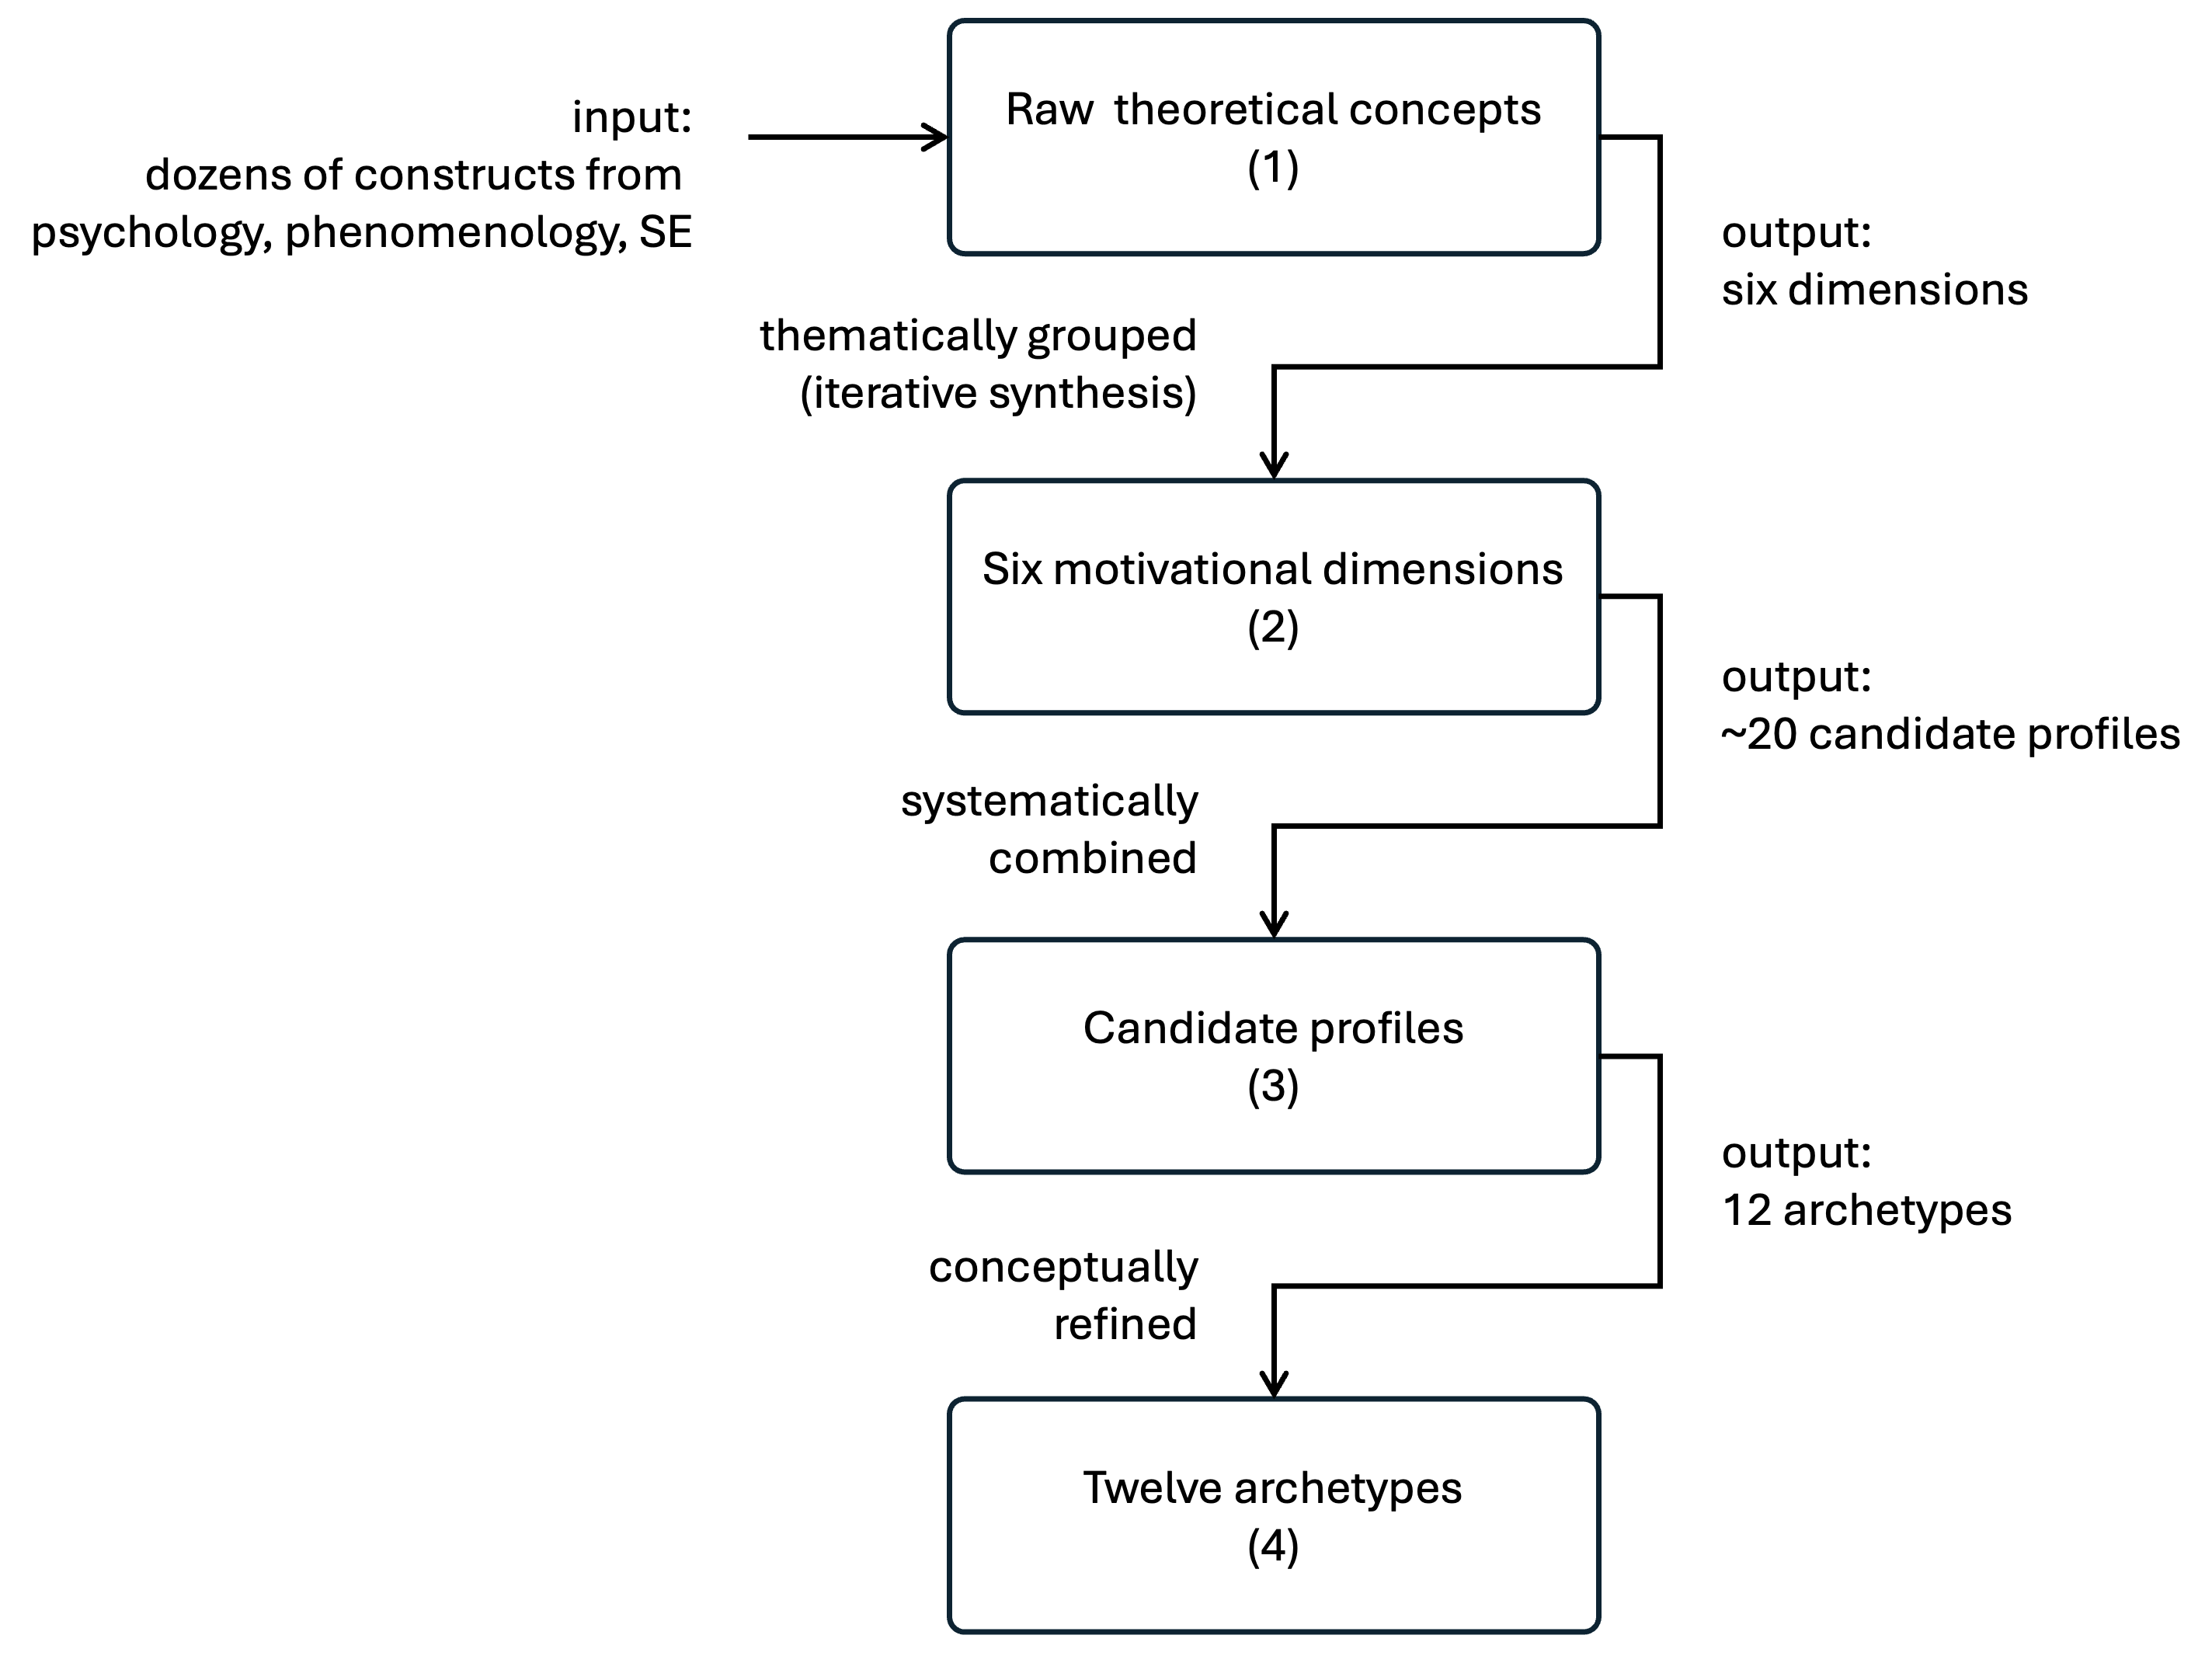
\includegraphics[width=0.75\linewidth]{images/pipeline.png}
    \caption{High-level pipeline for deriving the twelve archetypes. Raw theoretical constructs were 
    synthesized into six motivational dimensions, which were then systematically 
    combined into an initial set of candidate profiles. These profiles were refined 
    through iterative evaluation of coherence, distinctiveness, and redundancy, 
    yielding the final twelve archetypes.}
    \label{fig:pipeline}
\end{figure}

\subsection{Operationalizing the Motivational Dimensions}
The six motivational dimensions (Growth, Resolution, Coherence, Creation, 
Contribution, and Autonomy) were derived from four foundational components: 
values, reward sensitivity, cognitive style, and reinforcement history. These 
components are well established in psychology (e.g., \cite{deci1985intrinsic, 
kozhevnikov2007cognitive}) and are systematically linked to how individuals 
derive meaning and positive affect from cognitively complex work. Each dimension 
was treated as a continuous variable that represents sensitivity to a specific 
class of intrinsically rewarding experiences.

\subsection{Profiling Motivational Sensitivities}
To construct motivational profiles, we adopted a theory-driven approach 
analogous to persona construction in HCI rather than algorithmic clustering, 
which can produce opaque or unstable categories. Each profile represents a 
coherent pattern of sensitivities across the six dimensions and expresses a 
distinct "joy signature", a stable tendency in how practitioners interpret, 
value, and respond to aspects of software work. This approach ensured that the 
profiles aligned with both psychological principles and observations from 
developer-focused research (cf.~\cite{ford2015exploring}).

\subsection{Synthesizing Archetypes}
The synthesis followed several stages, illustrated in Fig.~\ref{fig:pipeline}. 
First, we compiled a broad set of raw theoretical constructs~(1) from 
psychology, phenomenology, and software engineering research. Through an iterative 
thematic synthesis, these constructs were distilled into the six motivational 
dimensions~(2). The dimensions were then systematically combined into 
theoretically plausible motivational configurations (e.g., high mastery + strong 
structure; high exploration + strong autonomy; high contribution + high 
relational sensitivity), producing an initial set of approximately 20 
\emph{candidate profiles}~(3). These candidates represented the conceptual space 
of motivational sensitivities rather than empirically observed behavioral 
clusters.

Each candidate was evaluated for \emph{internal coherence}, meaning that its 
motivational tendencies complemented rather than contradicted each other, and 
for \emph{distinctiveness}, ensuring that no two profiles described essentially 
the same motivational pattern. Profiles with extensive conceptual overlap were 
merged, while those with incompatible tendencies were removed. During 
approximately three cycles of synthesis and refinement, the candidate set was 
reduced to a stable set of twelve archetypes~(4).

This convergence was not arbitrary. The six dimensions do not combine freely: 
certain configurations are theoretically incompatible (e.g., simultaneously 
valuing strict structural coherence and unconstrained exploration), while 
others collapse into variations of the same motivational pattern. 
During synthesis, conceptual stability was achieved only for profiles that expressed
a clear \emph{dominant} motivational dimension, typically supported
by one or more \emph{secondary} tendencies. This constraint imposed structure on
the motivational space, preventing unconstrained combinatorial proliferation
and yielding a finite set of coherent motivational signatures. When incoherent
configurations were eliminated and overlapping profiles merged, the remaining
patterns converged into twelve psychologically meaningful archetypes. These twelve represent 
the distinct patterns that optimally balance dominance, complementarity, and 
coherence across the six-dimensional motivational space.

The complete synthesis procedure is summarized in Fig.~\ref{fig:detailed-pipeline}, 
which expands the high-level structure shown earlier in Fig.~\ref{fig:pipeline} 
into the full sequence of analytic, filtering, and encoding steps.

\begin{figure}[H]
    \centering
    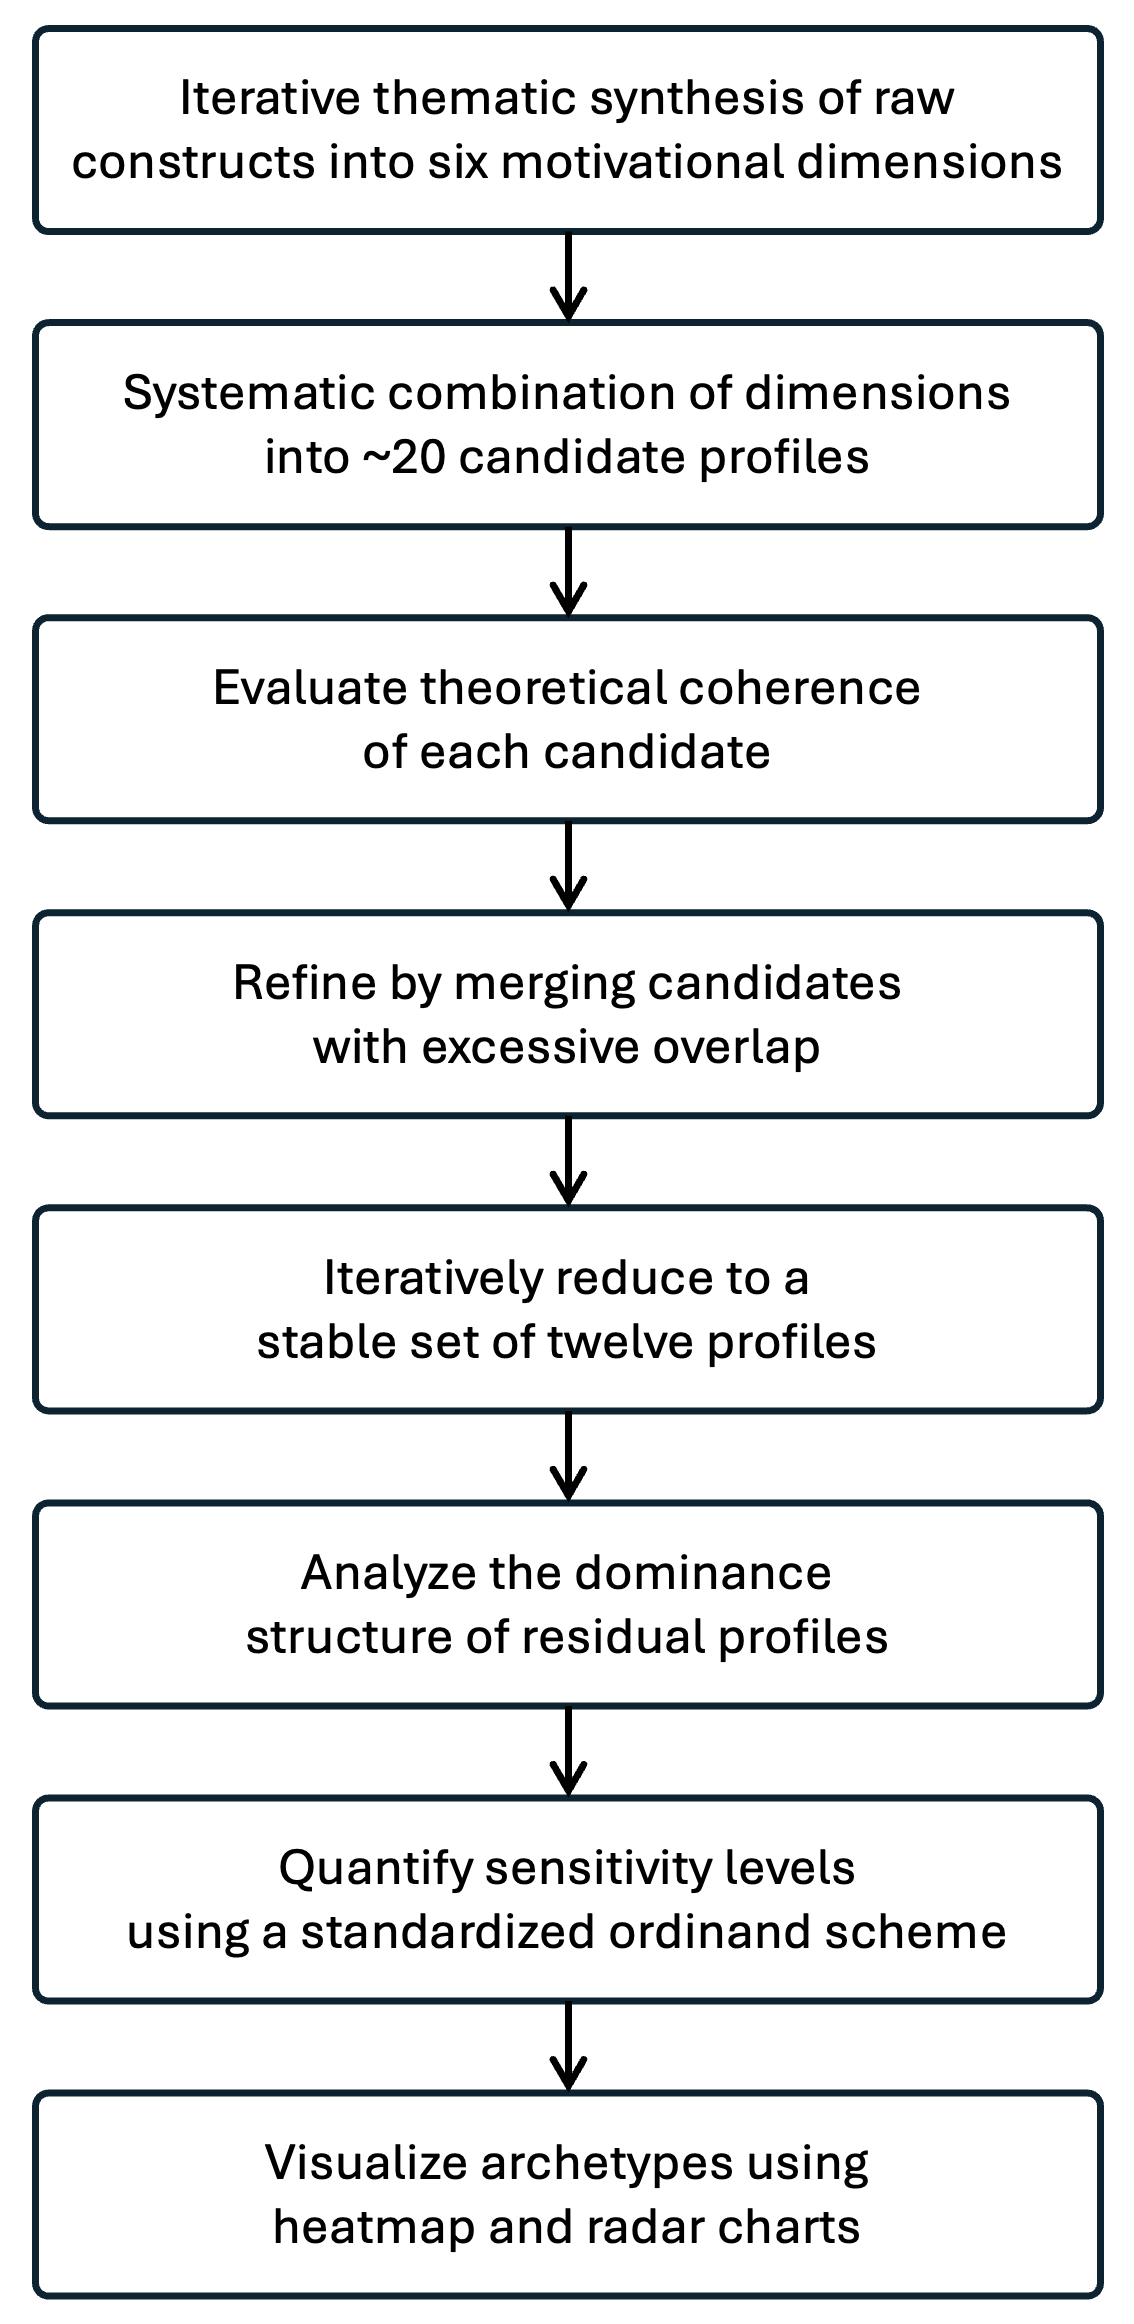
\includegraphics[width=0.4\linewidth]{images/detailed-pipeline.png}
    \caption{Detailed pipeline used to derive the twelve archetypes. Raw theoretical constructs were synthesized into six motivational dimensions, combined into candidate profiles, evaluated for coherence and distinctiveness, and iteratively refined. The final profiles were quantified using a standardized ordinal scheme and visualized through heatmap and radar charts.}
    \label{fig:detailed-pipeline}
\end{figure}





\smallskip
The synthesis drew on multiple theoretical sources, including intrinsic
motivation \cite{ryan2000selfdetermination}, reward sensitivity and individual
differences \cite{gray1987personality}, cognitive styles
\cite{messick1976personality}, flow theory \cite{csikszentmihalyi1990flow},
phenomenology of tool use \cite{heidegger1996being,ihde1990technology}, and
software engineering cognition \cite{parnin2011programmer}.
From these bodies of work, we selectively extracted constructs directly related
to experiential quality, agency, structure, exploration, contribution, and
coherence in cognitively demanding activities. These constructs formed the
conceptual input to the first stage of the synthesis pipeline. A summary of the
raw constructs used in this stage is provided in Table~\ref{tab:rawconcepts}.


\subsection{Visualizing Motivational Profiles}
\label{sec:profiles}

To generate the radar charts in Fig.~\ref{fig:joyradars}, the 
motivational structure of each archetype was translated into a numerical sensitivity profile on 
the six motivational dimensions. Because the typology is theory-driven 
rather than empirically clustered, these values were not obtained from data, but 
from structured conceptual analysis. Each archetype was characterized by a 
\emph{dominant} dimension, one or more \emph{secondary} tendencies, and, when 
appropriate, additional \emph{tertiary} influences. These assignments were 
expressed using the following ordinal mapping:

\begin{equation}
d_i =
\begin{cases}
1.0 & \text{if dimension } i \text{ is dominant},\\[4pt]
0.6 & \text{if dimension } i \text{ is secondary},\\[4pt]
0.3 & \text{if dimension } i \text{ is tertiary/supportive},\\[4pt]
0.0 & \text{if dimension } i \text{ is not characteristic}.
\end{cases}
\label{eq:mapping}
\end{equation}

To ensure transparency in how these profiles were operationalized, the 
qualitative motivational configuration of each archetype was translated into a 
standardized numerical pattern using Eq.~\ref{eq:mapping}. This produced a 
complete $12 \times 6$ sensitivity matrix, in which each archetype is assigned a 
dominant dimension (1.0), one or more secondary dimensions (0.6), optional 
tertiary supports (0.3) and non-characteristic dimensions (0.0). These values 
are not empirical measurements but structured theoretical assignments derived 
from the conceptual synthesis described earlier in this section. The matrix is 
reported in Table~\ref{tab:sensitivity} and serves as the basis for both the 
heatmap in Fig.~\ref{fig:heatmap} and the radar charts in 
Fig.~\ref{fig:joyradars}. All values were normalized to the range $[0,1]$ to 
support visual comparison.

\begin{figure}[H]
    \centering
    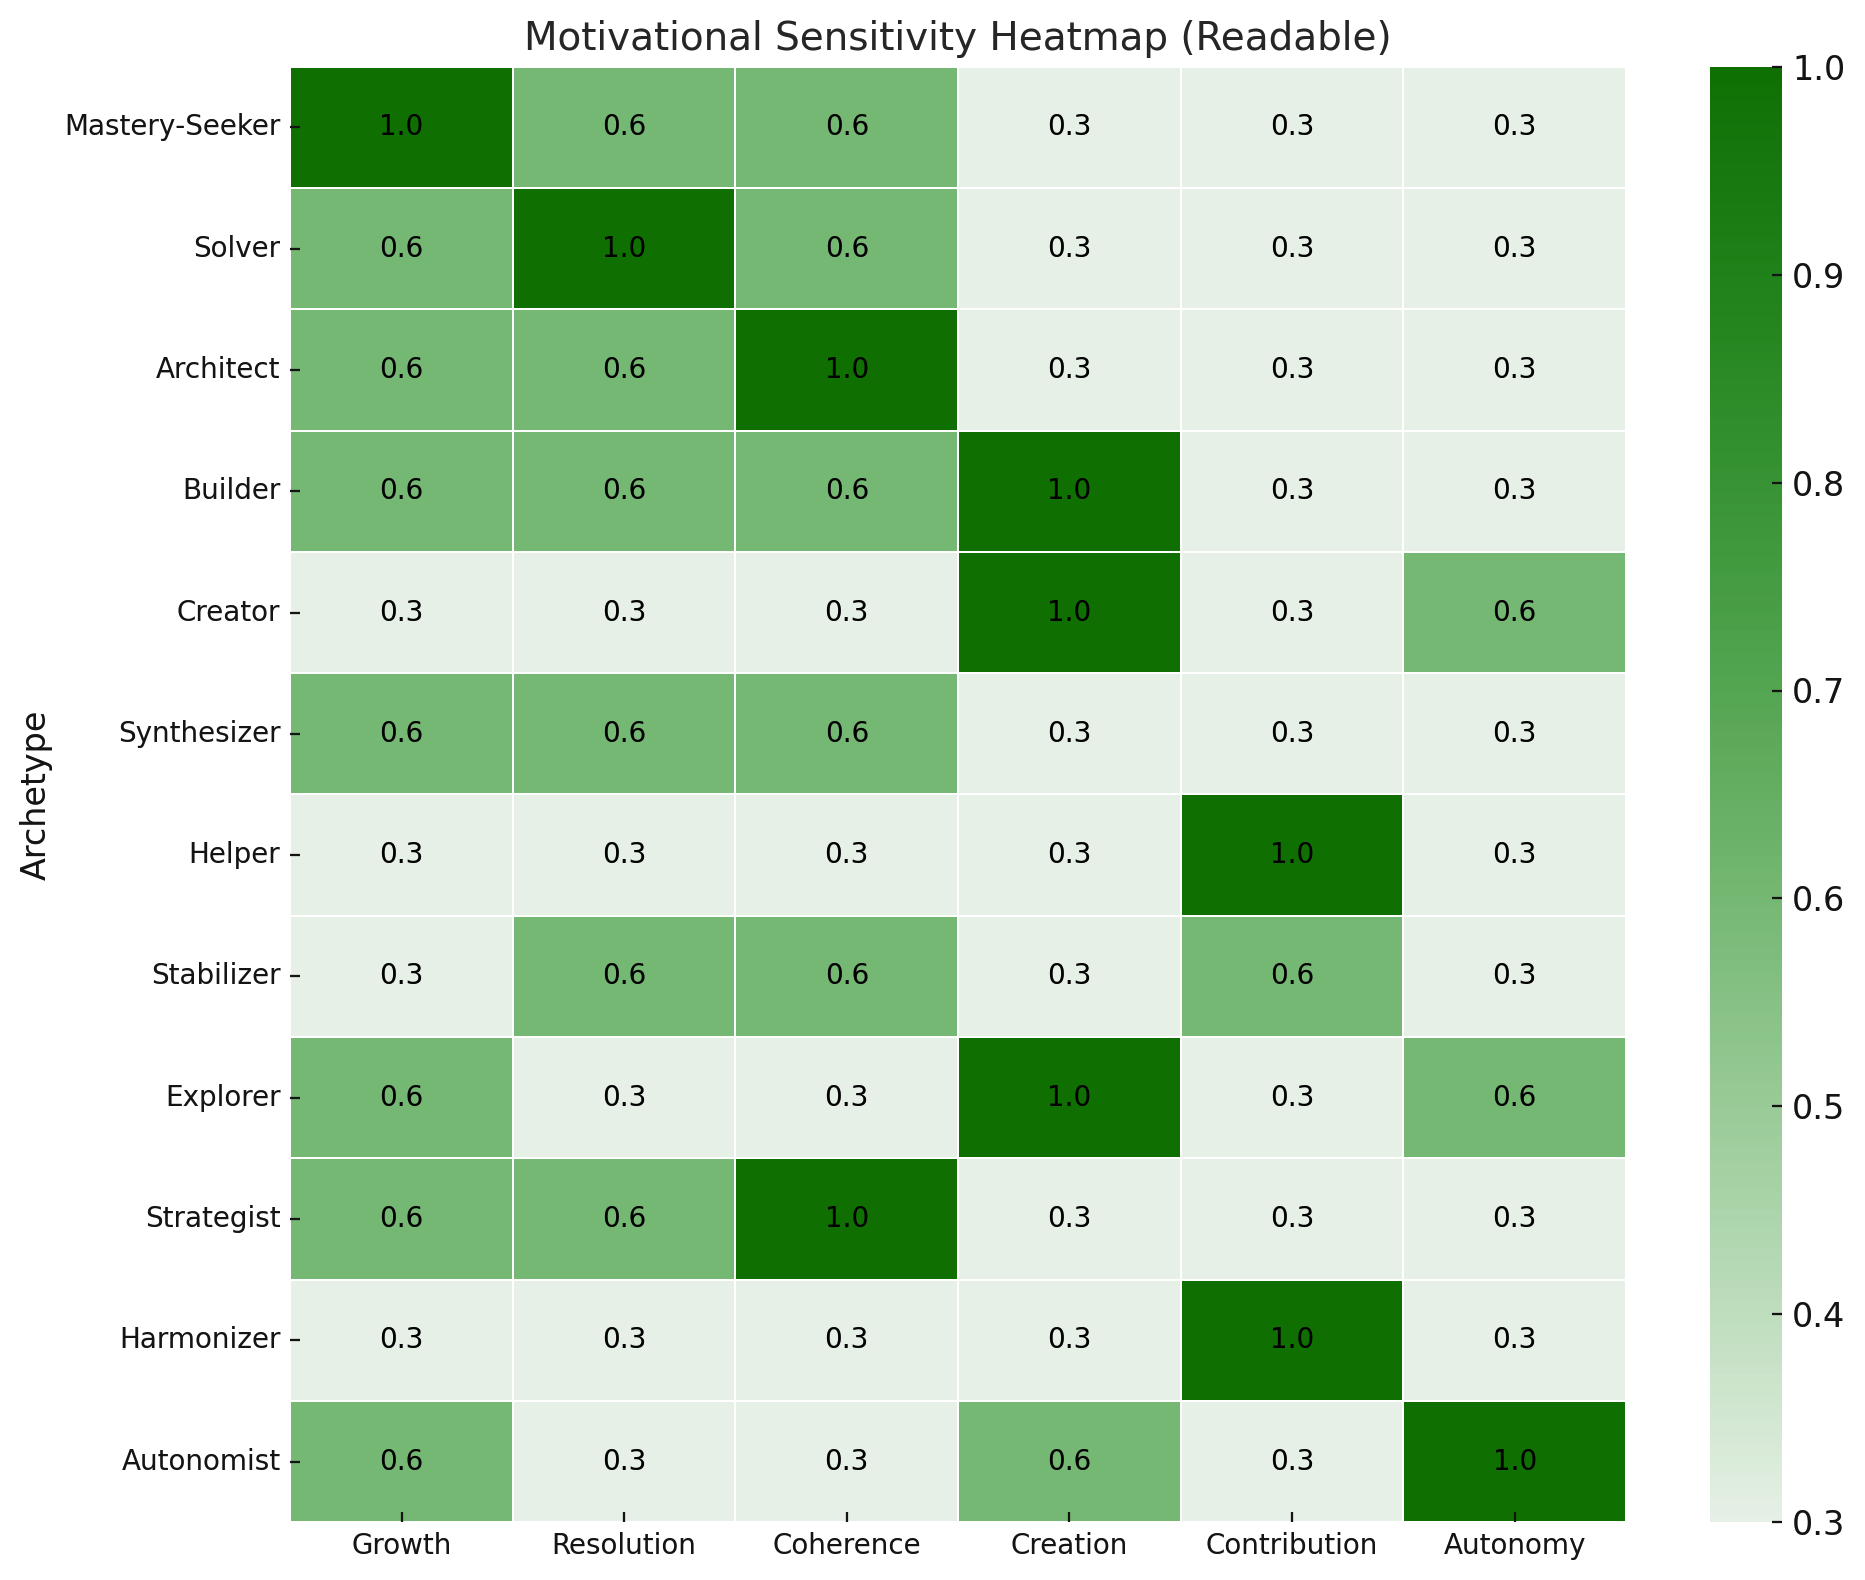
\includegraphics[width=\linewidth]{images/heatmap.png}
    \caption{Heatmap of the standardized sensitivity values used to construct 
    the twelve archetypes. Each cell indicates the motivational sensitivity of 
    a given archetype to one of the six dimensions (Growth, Resolution, 
    Coherence, Creation, Contribution, Autonomy). Values follow the ordinal 
    mapping defined in Eq.~\ref{eq:mapping} and correspond to the assignments 
    listed in Table~\ref{tab:sensitivity}. The heatmap provides a compact view 
    of the archetype space, highlighting how each configuration occupies a 
    distinct region of the motivational landscape.}
    \label{fig:heatmap}
\end{figure}

The heatmap in Fig.~\ref{fig:heatmap} offers a global view of the typology 
before the individual profiles are shown. It highlights dominant motivational 
tendencies as high-intensity regions, secondary tendencies as intermediate 
gradients, and non-characteristic dimensions as low-intensity cells. The radar 
charts in Fig.~\ref{fig:joyradars} then provide archetype-specific 
visualizations of these same profiles.

\subsection{Ensuring Coverage and Distinctiveness}
To validate the typology, we assessed its conceptual \emph{coverage}, ensuring 
that it spans the primary ways practitioners derive joy from software creation, 
and its \emph{distinctiveness}, ensuring that each archetype reflects a unique 
motivational configuration. Only profiles representing meaningfully different 
sources of joyful engagement were retained. The resulting typology, comprising Mastery-Seeker, Solver, Architect, Builder, Creator, Synthesizer, Helper, Stabilizer, Explorer, Strategist, Harmonizer, and Autonomist, offers sufficient granularity to represent the diversity of joyful engagement while preventing unnecessary proliferation of types.

These archetypes form the basis for the experiential model presented in 
Sect.~\ref{sec:dynamics}, which explains how transparency, flow, and 
motivational orientation dynamically interact to produce joyful software work. Together, the heatmap (Fig.~2) and the radar charts (Fig.~3) visualize the same 
underlying sensitivity matrix at different levels of granularity.



\section{The Twelve Archetypes of Joy in Software Creation}\label{sec:archetypes}


\begin{table}[H]
\centering
\caption{Standardized sensitivity values for the twelve archetypes across the six motivational dimensions. Dominant = 1.0, Secondary = 0.6, Tertiary = 0.3 (see Sect.~\ref{sec:method} and Eq.~\ref{eq:mapping}).}

\footnotesize
\resizebox{\linewidth}{!}{%
\begin{tabular}{lcccccc}
\toprule
\textbf{Archetype} & \textbf{Growth (G)} & \textbf{Resolution (R)} & \textbf{Coherence (C)} & \textbf{Creation (Cr)} & \textbf{Contribution (Co)} & \textbf{Autonomy (A)} \\
\midrule
Mastery-Seeker   & 1.0 & 0.6 & 0.3 & 0.0 & 0.0 & 0.0 \\
Solver           & 0.6 & 1.0 & 0.6 & 0.0 & 0.0 & 0.0 \\
Architect        & 0.3 & 0.6 & 1.0 & 0.0 & 0.0 & 0.3 \\
Builder          & 0.6 & 0.6 & 0.3 & 0.0 & 0.3 & 0.0 \\
Creator          & 0.3 & 0.0 & 0.0 & 1.0 & 0.6 & 0.3 \\
Synthesizer      & 0.3 & 0.6 & 1.0 & 0.6 & 0.3 & 0.0 \\
Helper           & 0.3 & 0.3 & 0.0 & 0.0 & 1.0 & 0.6 \\
Stabilizer       & 0.0 & 1.0 & 0.6 & 0.0 & 0.3 & 0.0 \\
Explorer         & 0.6 & 0.0 & 0.0 & 0.6 & 0.3 & 1.0 \\
Strategist       & 0.6 & 0.6 & 0.3 & 0.3 & 1.0 & 0.0 \\
Harmonizer       & 0.3 & 0.3 & 0.6 & 0.0 & 1.0 & 0.3 \\
Autonomist       & 0.0 & 0.0 & 0.0 & 0.3 & 0.3 & 1.0 \\
\bottomrule
\end{tabular}}
\label{tab:sensitivity}
\end{table}

The twelve archetypes represent distinct motivational configurations through which
practitioners experience joy during software creation. Each archetype integrates the 
six motivational dimensions introduced earlier, i.e., Growth, Resolution, Coherence, 
Creation, Contribution, and Autonomy, into a stable pattern of sensitivity. 
Although individuals rarely embody a single archetype exclusively, profiles 
provide interpretable "joy signatures" that capture recurring tendencies. 
Figure~\ref{fig:joyradars} illustrates the radar charts for all archetypes.
\begin{figure}[H]
  \centering
  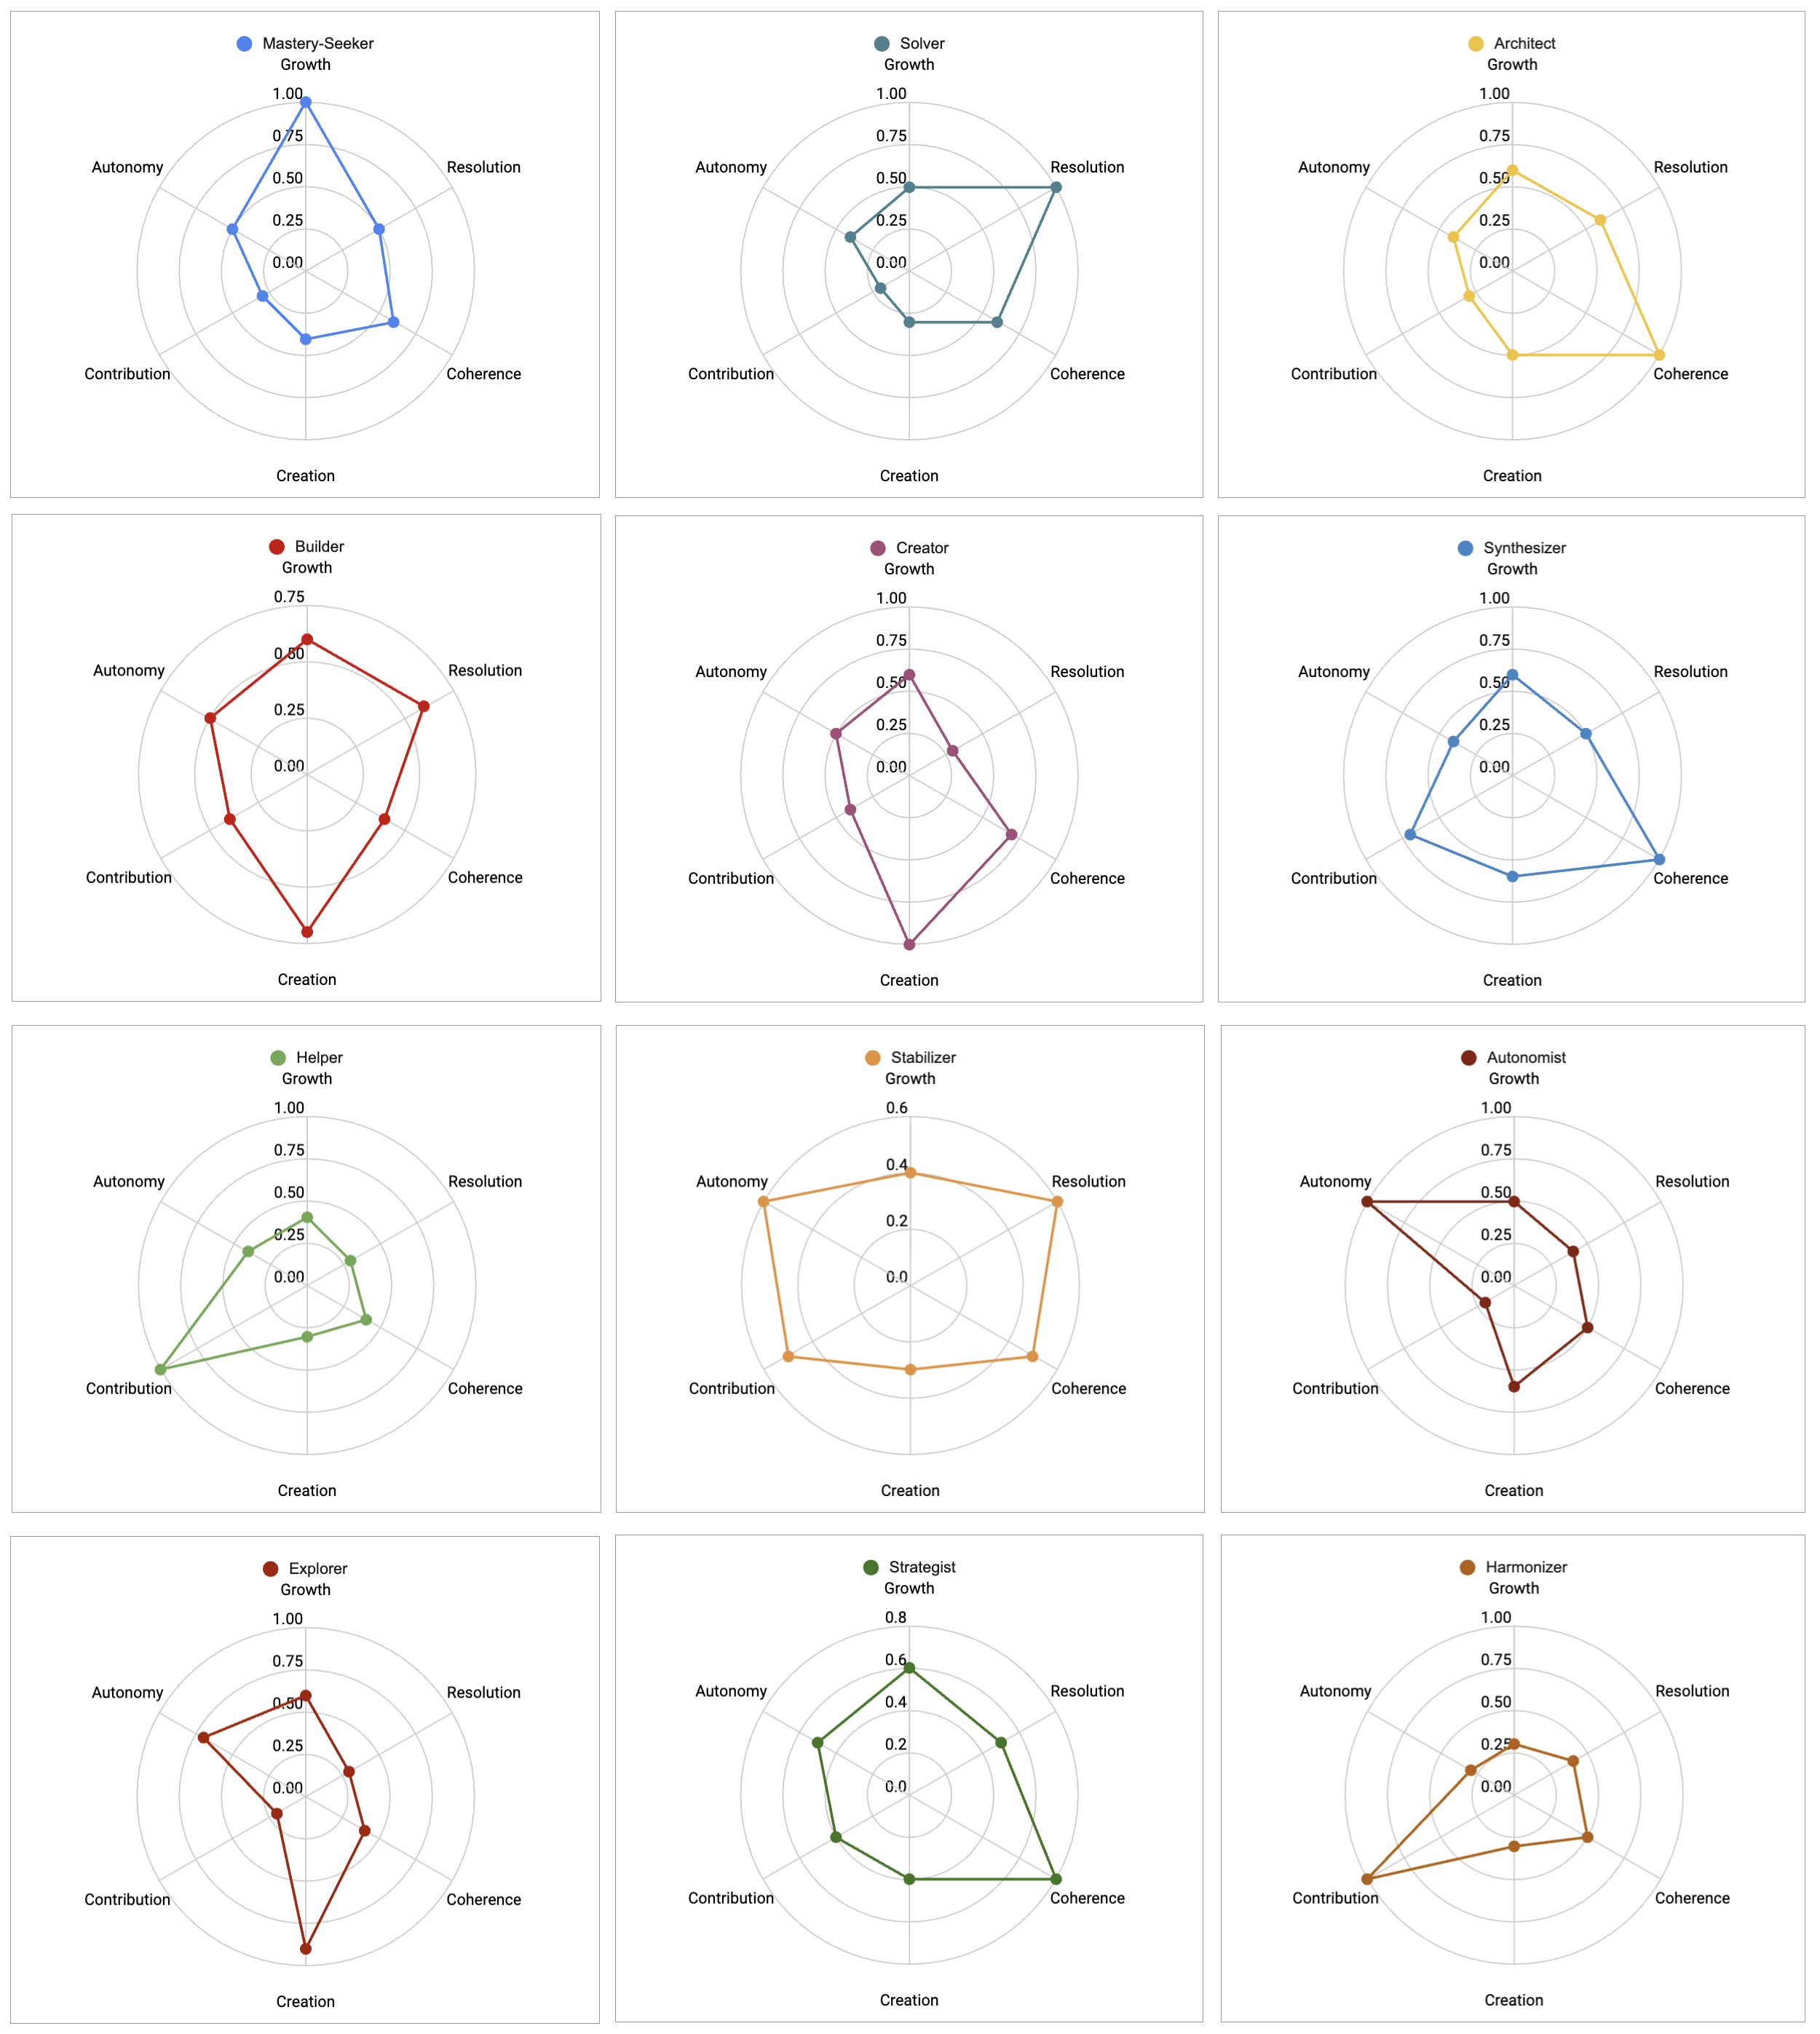
\includegraphics[width=\textwidth]{images/radar.png}
  \caption{Radar charts showing the motivational sensitivity profile of each 
archetype across the six dimensions. Values are derived using the ordinal 
mapping scheme defined in Sect.~\ref{sec:method} (dominant = 1.0, secondary = 
0.6, tertiary = 0.3; see equation~(\ref{eq:mapping})) and correspond to the 
standardized assignments reported in Table~\ref{tab:sensitivity}. These 
profiles provide theory-driven interpretive summaries of each archetype’s 
motivational configuration rather than empirically measured data.}
  \label{fig:joyradars}
\end{figure}
\smallskip
The model integrates the six motivational dimensions introduced in 
Sect.~\ref{sec:foundations} with the archetypal configurations derived in 
Sect.~\ref{sec:archetypes}, grounding the dynamics of joyful engagement in 
the interplay of individual sensitivities and environmental conditions.

\subsection{Mastery-Seeker}
Mastery-Seekers derive joy primarily from Growth. They are energized by learning,
skill development, and the acquisition of deeper conceptual insight. Joy arises
when tasks present challenges that stretch the competence without overwhelming it.
Resolution and Coherence support their engagement, but novelty is meaningful only
when it contributes to progression in mastery. Mastery-Seekers thrive in
environments that reward exploration of ideas, provide rapid performance
feedback, and expose them to progressively harder problems.

\subsection{Solver}
Solvers experience joy through Resolution: turning ambiguity into clarity and
closing gaps in understanding. They find satisfaction in debugging, refactoring,
and untangling complex problems. Flow for Solvers emerges when they can iteratively
test hypotheses and converge on elegant solutions. Coherence and Growth 
reinforce this engagement, but Creation is secondary unless it supports problem 
closure. They flourish in settings where problems are well-scoped and rapid 
feedback loops are available.

\subsection{Architect}
Architects derive joy from Coherence: creating systems in which structure,
constraints, and relationships form a unified whole. They are motivated by
conceptual clarity, pattern formation, and long-range consistency. Flow emerges
when they can work at the level of abstractions without disruptive contextual
shifts. Resolution and Autonomy support their engagement, while Contribution 
matters when the architecture impacts team alignment. They excel in roles that
involve system design, modeling, or reasoning about large-scale structure.

\subsection{Builder}
Builders experience joy through Creation grounded in concreteness. They find
satisfaction in making things work, for instance, implementing features, wiring components,
and seeing tangible progress. Flow arises from steady forward movement, where
tools remain predictable, and interruptions are minimal. Growth and Resolution 
support engagement, but conceptual elegance is secondary to functionality. 
Builders thrive in environments that allow for incremental construction, stable 
toolchains, and visible results.

\subsection{Creator}
Creators derive joy from open-ended Creation and expressive freedom. They excel
in generating new ideas, experimenting with alternatives and imagining 
possibilities. Flow arises from exploration unconstrained by rigid structure.
Autonomy amplifies their engagement, while Coherence matters only insofar
as it supports imaginative expression. Creators flourish in settings that allow
for ideation, prototyping, and conceptual play.

\subsection{Synthesizer}
Synthesizers are grateful to integrate diverse ideas into a coherent 
whole. Their engagement peaks when connecting perspectives, aligning 
constraints, or reconciling conceptual tensions. Coherence and Contribution 
reinforce their motivation, while Resolution supports refinement of 
emerging structures. They thrive in interdisciplinary work and collaborative 
design tasks where integration is central.

\subsection{Helper}
Helpers derive joy from Contribution: enabling others to succeed. They find
satisfaction in mentoring, improving practices, or removing obstacles for the
team. Flow arises when assisting others aligns with their technical engagement.
Resolution supports problem-solving for others, but personal novelty or autonomy 
is secondary. Helpers excel in collaborative environments, code review, 
documentation, and knowledge-sharing roles.

\subsection{Stabilizer}
Stabilizers experience joy through reliability, predictability, and long-term
maintenance of functioning systems. Their primary dimension is Contribution 
oriented toward system stability rather than interpersonal support. Flow 
comes from ensuring consistency, monitoring behavior, or preventing 
regressions. Resolution reinforces their work; novelty is valued only when it 
reduces future uncertainty. Stabilizers thrive in operational, QA, or 
maintenance-oriented contexts.

\subsection{Explorer}
Explorers derive joy from novelty, experimentation, and boundary-pushing.
Autonomy and Creation dominate their profile, with Growth emerging through 
self-directed discovery. Flow arises when constraints are minimal and 
uncertainty is an invitation rather than an obstacle. Coherence matters only 
after the exploration produces insight. Explorers thrive in research, prototyping,
and experimental tool work.

\subsection{Strategist}
Strategists experience joy from long-range coherence: anticipating consequences,
weighing trade-offs, and shaping trajectories. They integrate Coherence, 
Autonomy, and Contribution, derived satisfaction from influencing the direction of the system
. Flow emerges in complex planning tasks or architectural evolution.
Resolution supports decision-making, but novelty matters only in the service of 
strategic clarity. Strategists thrive in leadership, architecture evolution, 
and high-level design.
\begin{figure}[H]
    \centering
    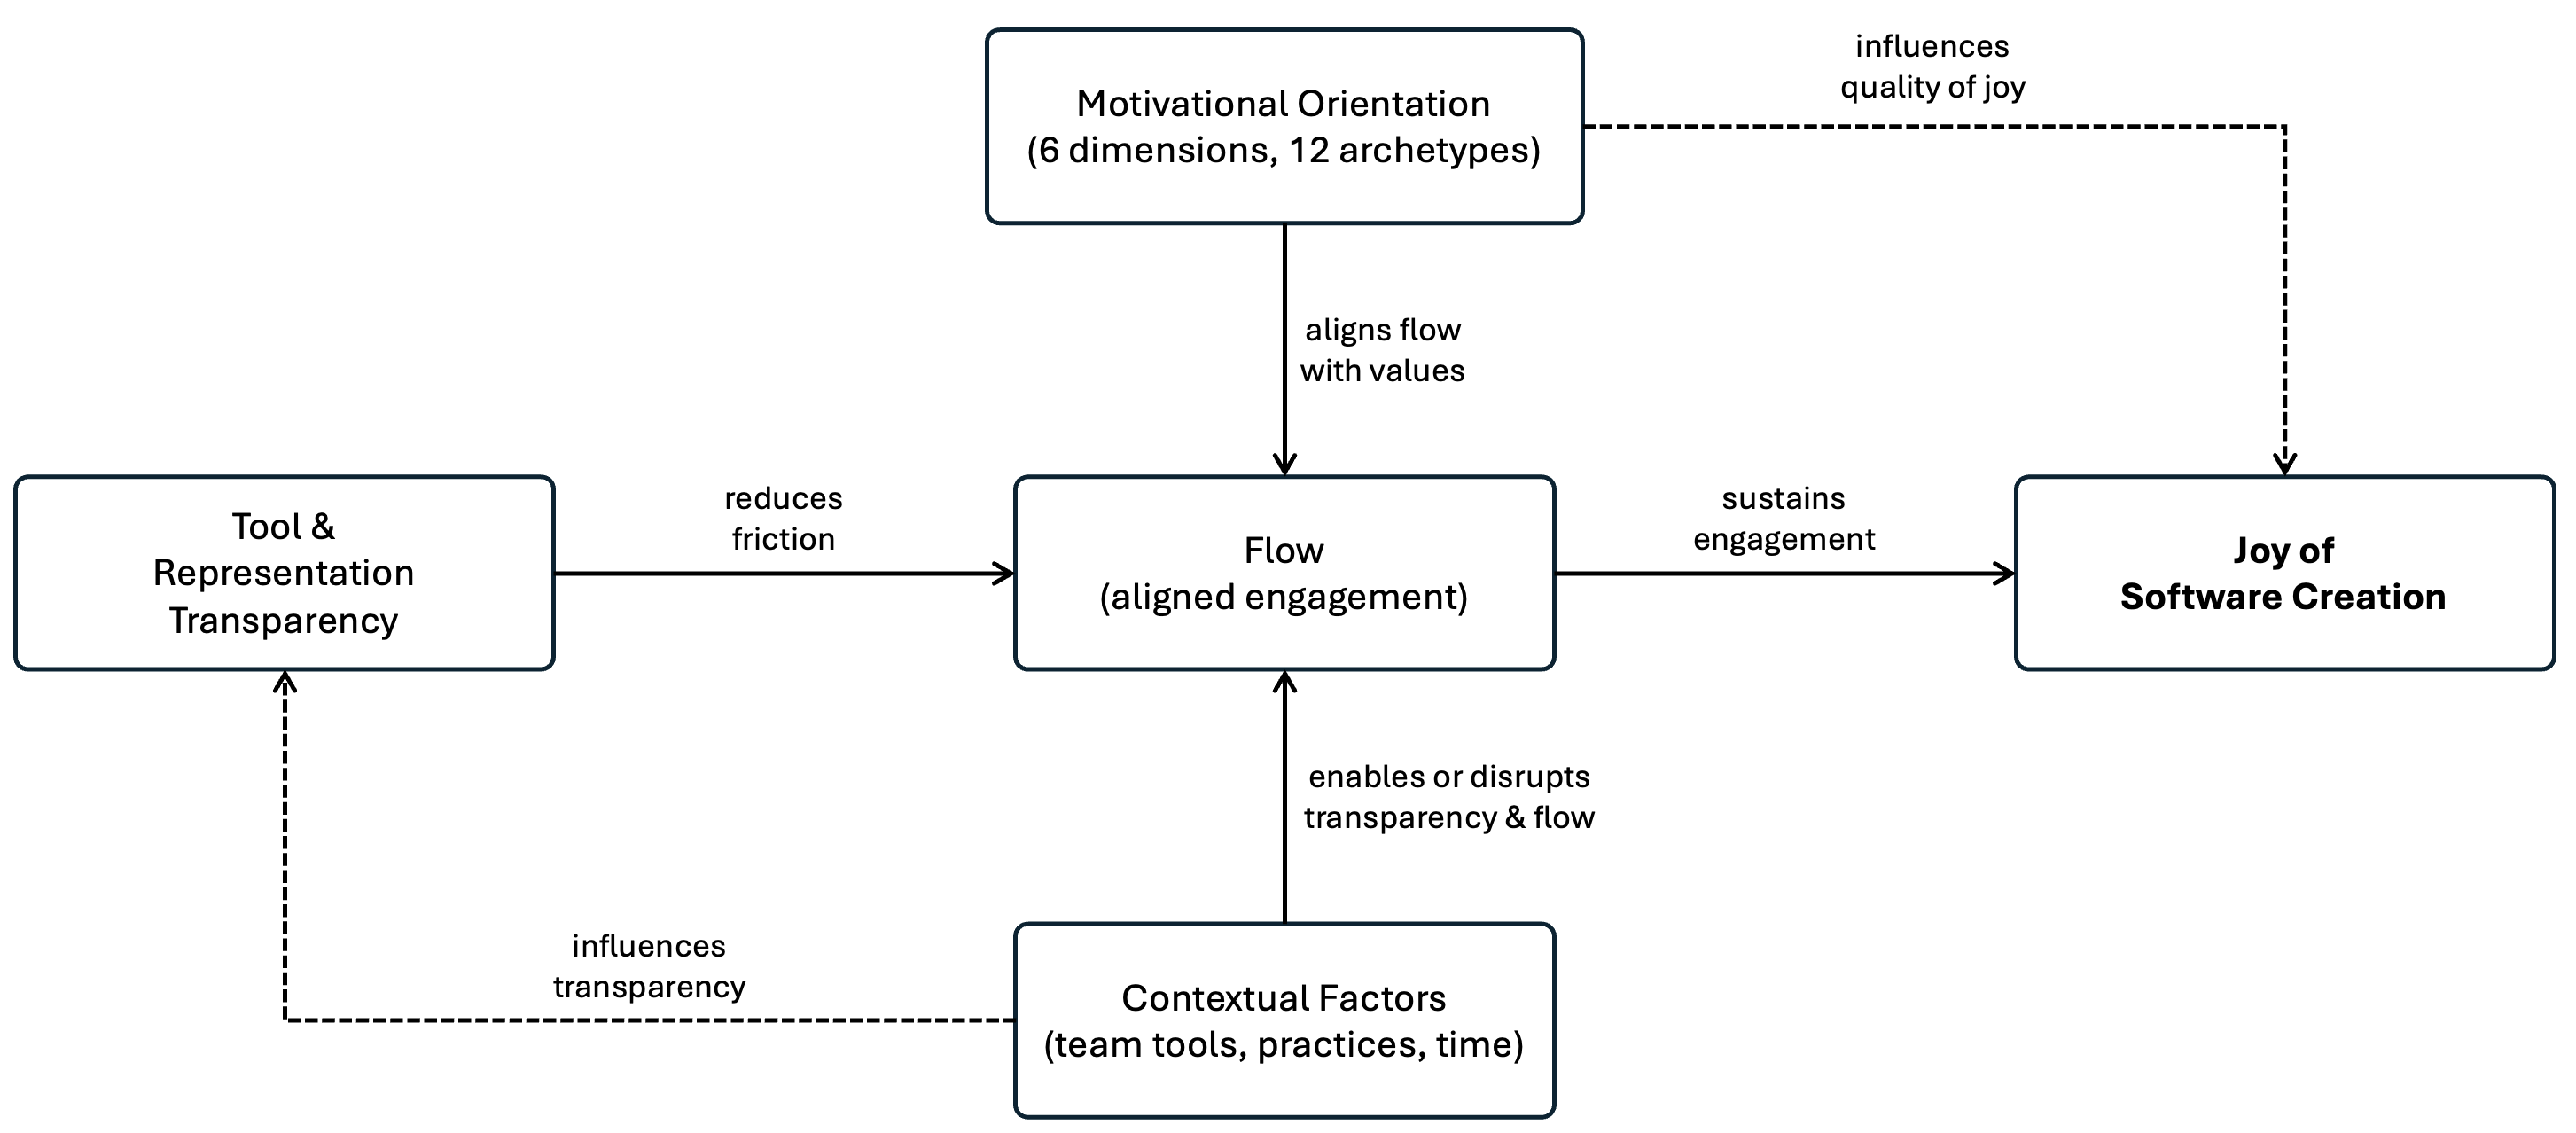
\includegraphics[width=.95\linewidth]{images/dynamics.png}
  \caption{Conceptual model of the dynamics of joy in software creation. 
  Transparency enables flow by reducing friction; motivational orientation 
  determines whether flow becomes joyful; contextual factors shape the 
  stability and quality of this interaction.}
  \label{fig:dynamics-of-joy}
\end{figure}
\subsection{Harmonizer}
Harmonizers derive joy from balancing technical, interpersonal, or
organizational tensions. They are sensitive to Contribution, Coherence, and Resolution
simultaneously and find satisfaction when systems, teams, and practices align.
Flow emerges in mediating competing constraints or integrating stakeholder 
needs. Harmonizers excel in roles requiring facilitation, coordination, 
and socio-technical negotiation.

\subsection{Autonomist}
Autonomists experience joy primarily through Autonomy: self-direction, control 
over workflow, and freedom from unnecessary constraints. Flow emerges in 
independent tasks with clear objectives and minimal external interference.
Creation and Resolution support their engagement when self-determined. 
Autonomists thrive in environments that provide flexibility, trust, and space 
for individualized workflows.

\section{Modeling the Dynamics of Joy}\label{sec:dynamics}

This section integrates the elements introduced earlier into a unified account 
of how joy arises and fluctuates during software creation. Rather than treating 
joy as a static property of individuals or tasks, we conceptualize it as an 
emerging phenomenon produced by the interaction of transparency, flow, 
motivational orientation, and contextual factors. The model explains both the 
shared mechanisms that underpin joyful participation and the individual differences 
captured by the archetypes in Sect.~\ref{sec:archetypes}.

\subsection{Core Components}
Four components form the basis for joyful participation in software work. 
The first is \textit{transparency}, which occurs when tools and representations 
recede from attention and allow practitioners to focus on the task rather than 
the mediating interface. When transparency is high, cognitive and 
phenomenological friction is reduced, enabling a smoother progression of thought 
and action.

The second component is \textit{flow}, the state of deep involvement in which 
attention is fully absorbed and the action--feedback loop becomes seamless. 
Flow emerges when the challenge--skill balance is appropriate and when feedback 
is immediate and interpretable.

The third component is \textit{motivational orientation}, which determines what 
aspects of the software work feel rewarding. As described in Sect.~\ref{sec:orientations}, 
motivational orientation arises from an individual's values, reward 
sensitivities, cognitive style, and reinforcement history. The six motivational 
dimensions, i.e., Growth, Resolution, Coherence, Creation, Contribution, and Autonomy, 
shape the experiences within flow that are interpreted as joyful.

Finally, \textit{contextual factors} such as team structures, development 
practices, time pressure, and tool ecosystems modulate both the probability of 
achieving transparency and the stability of flow once achieved.

\subsection{Dynamic Interactions}
Joy emerges from the interaction of these components. Transparency establishes 
the preconditions for engagement by reducing friction and stabilizing the 
action--feedback loop. When these conditions hold, practitioners are more 
likely to enter flow. Whether flow is subsequently experienced as joy depends 
on how well the characteristics of the activity align with the individual's 
motivational orientation. For example, a Solver experiences joy when flow is 
driven by convergence and clarity, while a Creator may feel joyful when flow 
supports exploration and generativity. Conversely, misalignment—such as high 
structure for an Explorer or high uncertainty for a Stabilizer—may allow flow 
but not joy.

Contextual factors modulate the whole process. Interruptions may disrupt flow 
for archetypes who rely heavily on continuity (e.g., Architects, Strategists), 
while rich collaborative environments may amplify joy for archetypes motivated 
by Contribution (e.g., Helpers, Harmonizers). Thus, joy is not only a function 
of individual traits or environmental conditions but also of the dynamic interplay 
between them.

The resulting model, summarized in Fig.~\ref{fig:dynamics-of-joy}, describes 
how transparency enables flow, how flow becomes joyful through motivational 
alignment, and how context shapes these dynamics. This provides a conceptual 
foundation for the design implications discussed in the next section.



\section{Typology Diagram and Cross-Archetype Analysis}\label{sec:typology}
Building on the experiential model in Sect.~\ref{sec:dynamics} and the archetypes 
defined in Sect.~\ref{sec:archetypes}, we outline the design implications that 
address both the shared cognitive mechanisms underlying joyful participation and 
the individual differences that shape how joy manifests across practitioners.

The twelve archetypes introduced in Sect.~\ref{sec:archetypes} provide a fine-grained account of
how different practitioners experience joy in software creation. While each
archetype represents a distinct motivational configuration, they also exhibit
systematic relationships that can be organized into a higher-order typology.
This section presents a conceptual map of the archetype space and analyzes
cross-archetype patterns that clarify the structural logic of the typology.
Rather than relying on quantitative clustering, the map is derived through a
theory-driven synthesis \cite{cooper2004inmates, pruit2006persona}, guided by 
the six motivational dimensions and their relative importance within each
profile.

\subsection{A Two-Dimensional Map of Motivational Orientation}

Figure~\ref{fig:typology-map} positions the archetypes along two emergent
axes that capture the most prominent sources of variation. The horizontal axis
contrasts \emph{Structure-Driven} versus \emph{Exploration-Driven}
motivations. Structure-Driven archetypes find joy in coherence, predictability,
and resolution, while Exploration-Driven archetypes derive joy from novelty,
open-ended creation, and autonomy.

The vertical axis contrasts \emph{Individual-Centric} versus
\emph{Contribution-Centric} orientations. Individual-Centric archetypes derive
joy primarily from personal mastery, autonomy, or expressive creation,
whereas Contribution-Centric archetypes derive joy from enabling others,
stabilizing systems, or aligning team practices.

This two-dimensional representation organizes the archetypes into a coherent
semantic space that clarifies their relationships and distinguishes broad
families of joyful engagement.

\subsection{Clusters and Families of Archetypes}

This mapping delineates four coherent clusters:
\paragraph{Systemic Thinkers (Structure-Driven, Individual-Centric)}
    Architect, Strategist, Synthesizer.  
    These archetypes derive joy from coherence, conceptual clarity, and
    long-range structure. They favor environments that offer stability,
    continuity, and time for deep reasoning.

\paragraph{Exploratory Creators (Exploration-Driven, Individual-Centric)}
    Creator, Explorer, Autonomist.  
    Their joy comes from autonomy, experimentation, and generative work.
    They thrive in contexts that minimize constraints and allow free-form
    exploration.
    
\paragraph{Collaborative Contributors (Structure-Driven, Contribution-Centric)}
    Helper, Harmonizer, Stabilizer.  
    These archetypes find joy in work that supports others or strengthens
    socio-technical cohesion. They prefer environments with rich
    interpersonal interaction or well-defined team workflows.

\paragraph{Problem-Oriented Drivers (Exploration-Driven, Contribution-Centric)}
    Solver, Builder, Mastery-Seeker.  
    Although individually motivated, they are oriented toward progress,
    closure, and pragmatic impact. Joy arises from making problems disappear, building solutions, or continuously improving competence.

\smallskip
These clusters highlight how apparently different archetypes share deeper
motivational commonalities. For instance, Solvers and Mastery-Seekers differ
in their primary emotional drivers (clarity vs.\ growth), yet both thrive on
progress and incremental advancement. Similarly, Helpers and Stabilizers both
prioritize Contribution but diverge on whether their focus is interpersonal or
technical.

\subsection{Tensions and Complementarities}

The typology also reveals significant tensions between archetypes.   Explorers and Stabilizers occupy opposite poles: the former seek novelty and freedom, while the latter find joy in predictability and system reliability. Creators and Architects may collaborate effectively but differ in their tolerance for ambiguity: what excites a Creator may frustrate an Architect.

Complementarities are equally important. Builders and Strategists share a natural synergy, as the former provide the incremental implementation momentum that enables the latter's long-range plans. Harmonizers and Architects complement each other by integrating technical and human constraints into coherent socio-technical systems.

Recognizing these dynamics is essential to understand how joy emerges in collaborative environments and how teams can be structured to support diverse motivational orientations.

\subsection{Implications of the Typology}

The typology clarifies that the experience of joy is not arbitrary but structured: archetypes cluster around stable motivational logics, and their relationships can be predicted by examining the six motivational dimensions. This understanding enables a more intentional design of tools, workflows, and collaboration structures, as elaborated in Sect.~\ref{sec:design}. By recognizing affinities and tensions of archetypes, organizations can better support individual well-being and team performance, while toolmakers can design environments that align with diverse motivational profiles.

\begin{figure}[H]
    \centering
    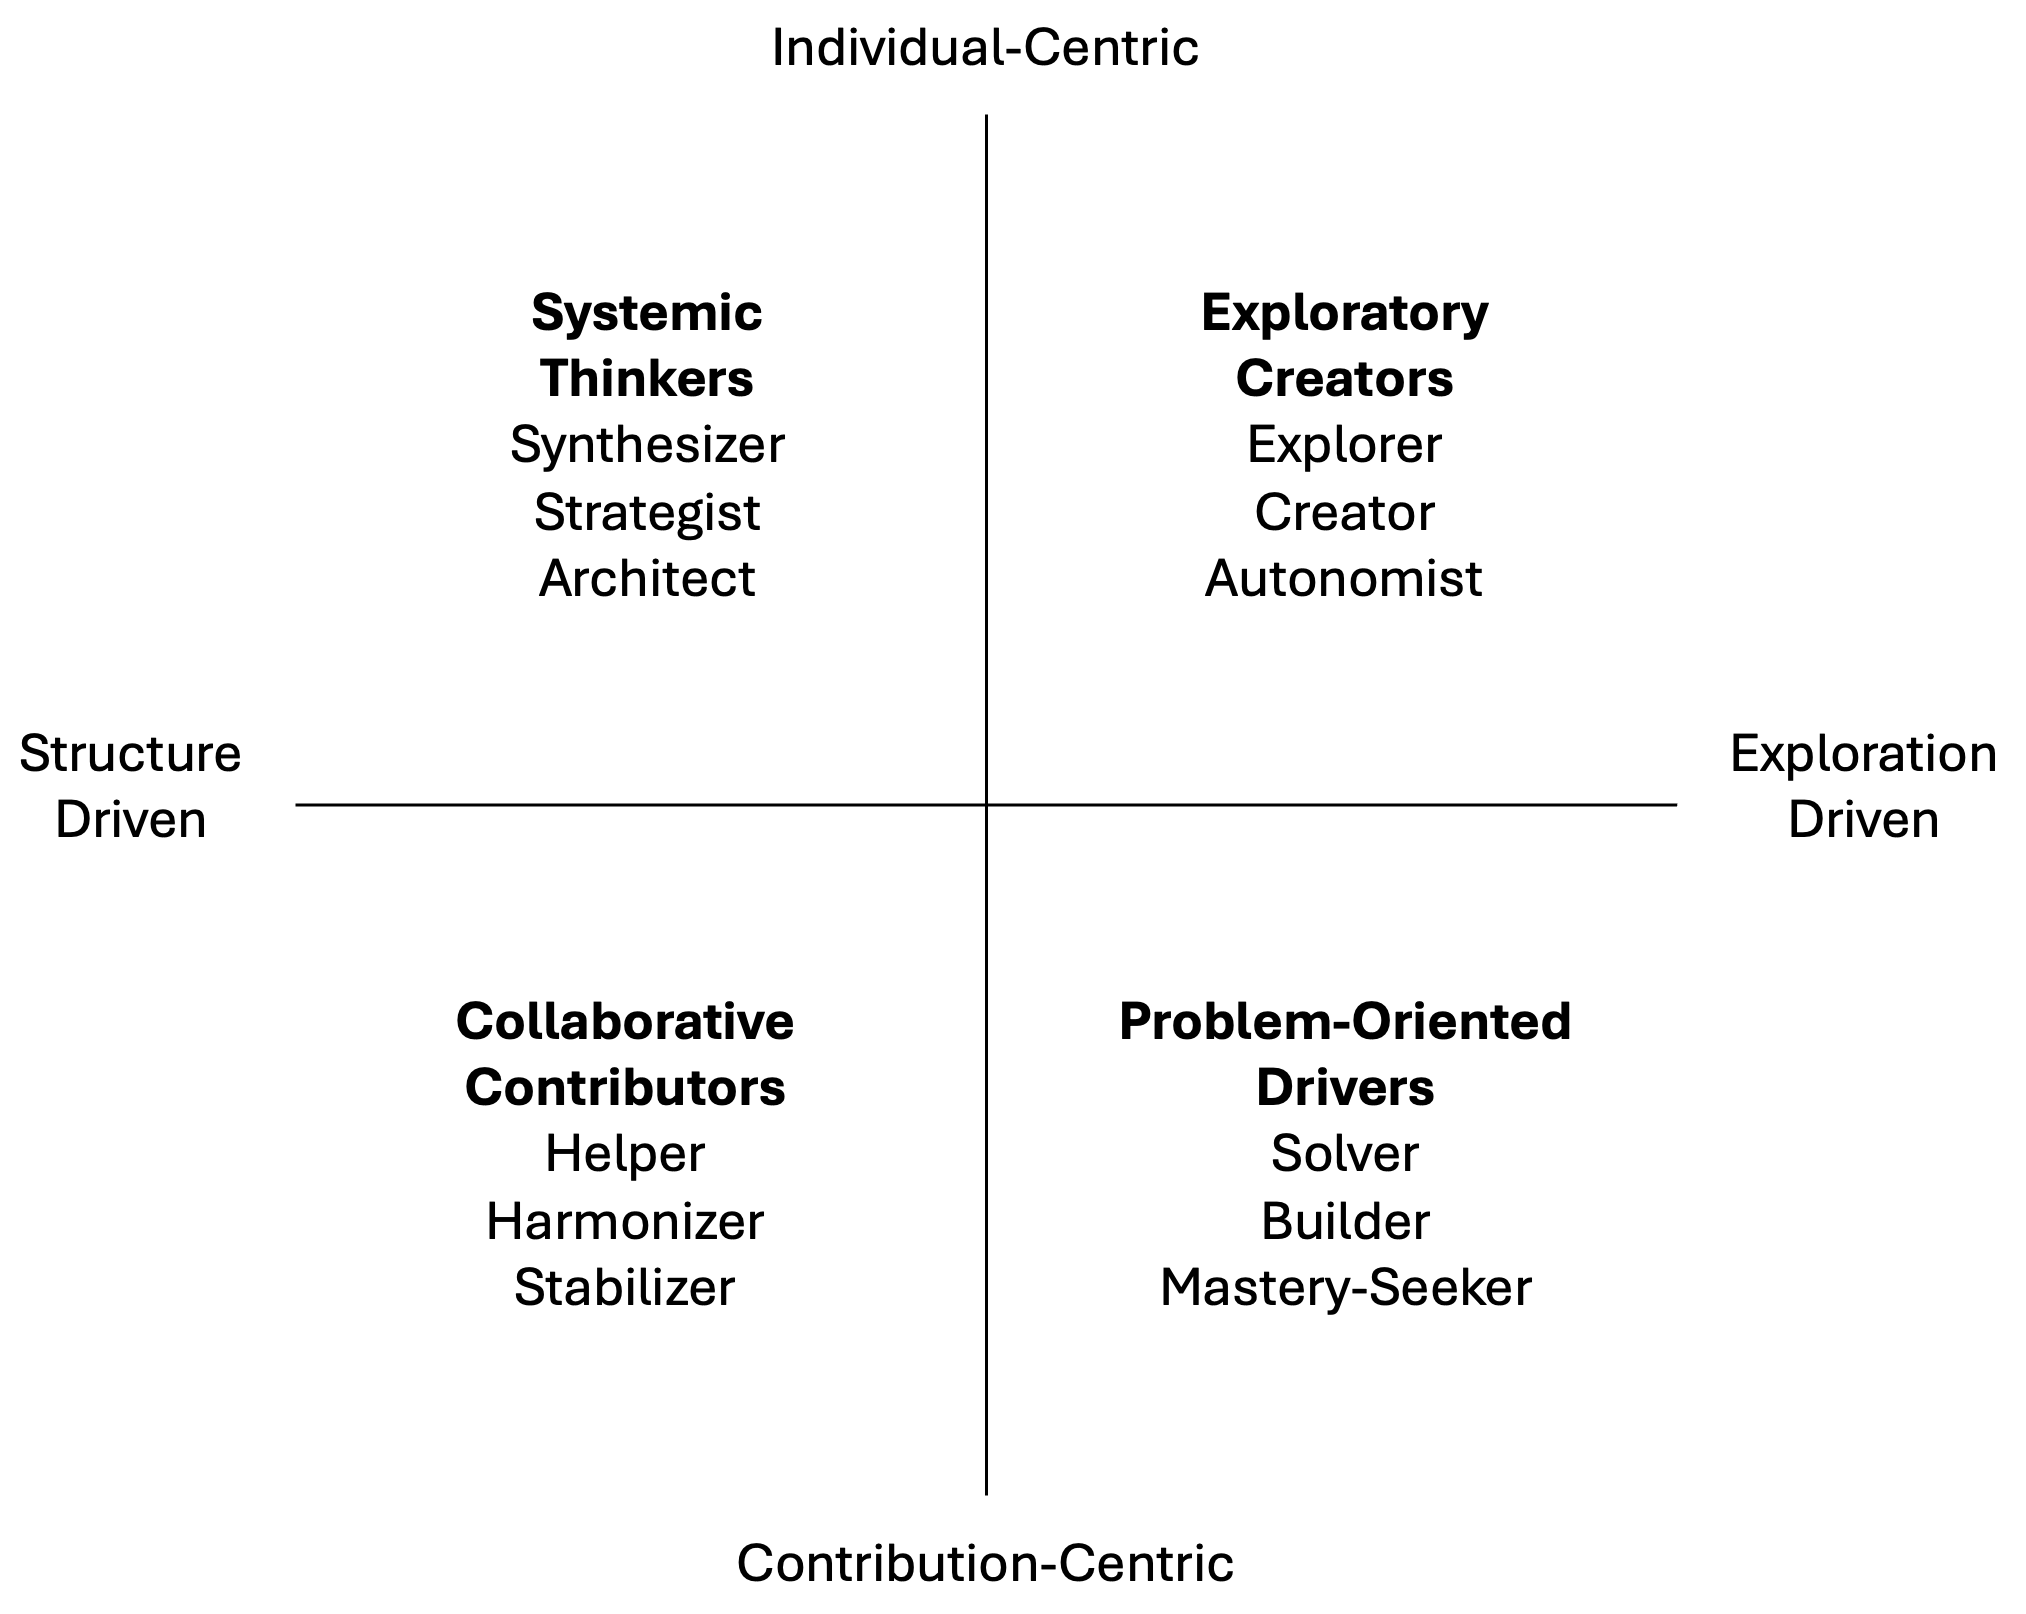
\includegraphics[width=0.75\linewidth]{images/typology-map.png}
    \caption{A conceptual map of the twelve archetypes, organized along two
  emergent axes: Structure-Driven vs.\ Exploration-Driven motivations
  (horizontal), and Individual-Centric vs.\ Contribution-Centric orientations
  (vertical). Clusters reveal four families of joyful engagement.}
     \label{fig:typology-map}
\end{figure}

%%%

\section{Implications for Design}\label{sec:design}
The archetypes and model are intended as analytical tools that support reflection,
reasoning about design choices, and alignment decisions rather than prescriptive
classifications.
The model developed in Sect.~\ref{sec:dynamics} and the typology presented in
Sect.~\ref{sec:typology} have direct implications for the design of software
tools, workflows, and socio-technical environments. Because joy emerges from the
interaction of transparency, flow, and motivational orientation, design must
take into account both the shared cognitive mechanisms that support frictionless
engagement and the individual differences that shape how that engagement becomes
meaningful.

To provide a high-level overview of these implications before elaborating on 
them in detail, Table~\ref{tab:design-implications} summarizes the main design 
considerations derived from our analysis. The table organizes the implications 
into four complementary focal areas: reducing friction and enhancing 
transparency, accommodating motivational diversity, structuring supportive 
socio-technical environments, and aligning tool affordances with contextual and 
individual needs. These categories collectively represent the core principles 
that guide the translation of our theoretical framework into actionable design 
guidance.

\begin{table}[t]
\centering
\caption{Summary of Design Implications for Supporting Joy in Software Creation}
\label{tab:design-implications}
\renewcommand{\arraystretch}{1.25}
\footnotesize
\begin{tabularx}{\linewidth}{lX}
\hline
\textbf{Design Focus} & \textbf{Key Implications} \\
\hline

\textbf{Transparency} \&\\ \textbf{Friction Reduction} & Minimize cognitive and phenomenological friction; reduce context-switching; simplify visual and textual noise; stabilize feedback loops; ensure predictable interactions; support continuity of thought; provide representations aligned with the cognitive grain of the task. \\

\textbf{Motivational Diversity} &
Support configurable workflows (structured vs.\ free-form); offer multiple 
representational views; adaptively surface features suited to motivational 
profiles; enhance opportunities for contribution (mentorship, 
knowledge-sharing); preserve autonomy through customization and local control. \\

\textbf{Socio-Technical} \\ \textbf{Environment} &
Balance challenge and skill; respect attentional rhythms (focus vs.\ 
collaboration); provide role flexibility; create teams with complementary 
archetypes; adapt workflows and practices rather than individuals to 
accommodate cognitive diversity. \\

\textbf{Holistic Alignment} &
Recognize that joy emerges only when motivational needs, tool affordances, and 
organizational conditions are aligned; design for continuity, autonomy, 
contribution, or exploration according to the archetype. \\
\hline
\end{tabularx}
\end{table}

Across archetypes, transparency is a universal prerequisite for sustained 
engagement. Tools should therefore minimize cognitive and phenomenological 
friction by reducing forced context-switches, lowering extraneous cognitive 
load, and providing stable, predictable interaction loops. Achieving this 
requires simplifying visual and textual noise, offering consistent 
representational idioms, and optimizing layouts for rapid interpretation. It 
also depends on stabilizing feedback loops so that edits, commands, and actions 
produce immediate, reliable, and interpretable responses. Supporting continuity 
of thought is equally important: low-disruption navigation, history-aware 
editing, and interaction modalities that minimize interruptions help 
practitioners maintain the cognitive momentum necessary for meaningful 
engagement. Finally, tools must align their abstractions and views with the 
cognitive grain of the task, ensuring that representations fit naturally with 
user’s reasoning processes (cf.~abstraction as cognitive alignment 
\cite{green1996usability, kramer2007abstraction}). These are not merely 
usability concerns; they establish the experiential preconditions under which 
flow can emerge. By systematically reducing friction, designers create 
environments in which practitioners can more easily align intentions, actions, 
and feedback: an alignment fundamental to the experience of joy.

\section*{Threats to Validity}
The contributions of this paper are based on a theory-driven synthesis rather than on empirical clustering or behavioral observation, which introduces several limitations. First, the construction of the six motivational dimensions and the twelve archetypes relies on conceptual analysis and expert interpretation. Although the synthesis process is transparent and follows an explicit pipeline, independent researchers could produce partially different groupings or labels. The absence of inter-rater procedures or triangulation limits reproducibility.

Second, the ordinal sensitivity values used for the visualizations are not derived from data, but rather from a structured theoretical mapping. The selected levels are conceptually justified but remain somewhat arbitrary, and alternative parameterizations might generate slightly different profiles or visual emphases. This affects the precision of the radar charts and heatmap, although not the underlying conceptual distinctions.

Third, the typology assumes relatively stable motivational orientations. In practice, developers may exhibit multiple tendencies or shift between orientations depending on task demands, experience, or organizational context. Although the model acknowledges variability, the archetypes function as idealized patterns that may not fully capture all individual trajectories.

Finally, the model has not yet been empirically validated. As a theory-building
contribution, the value of the proposed archetypes and model lies in explanatory
coherence and analytical usefulness rather than empirical completeness. Future
work should examine whether dimensions and archetypes correspond to
experienced patterns of joy in real software development settings, whether
developers self-identify consistently with the profiles, and whether the
proposed relationships between transparency, flow, and motivational orientation
hold in practice.

These limitations do not undermine the value of the conceptual framework, but they clarify the scope of the claims and motivate the need for empirical studies that can test, refine, or expand the theory.

\section{Conclusion}\label{sec:conclusion}
This paper examined the phenomenon of joy in software creation, arguing that
joyful engagement arises from the interaction of transparency, flow, and
motivational orientation. We developed a theoretical model that clarifies how
these mechanisms jointly structure the experiential quality of software work,
and we articulated a typology of twelve archetypes that capture distinct
motivational pathways toward joy. These contributions are based directly on the
six motivational dimensions introduced in Sect.\ref{sec:foundations}, the model
presented in Sect.\ref{sec:dynamics}, and the typology synthesized in
Sect.~\ref{sec:method}. Together, they provide a unified account of the
dynamics underlying joyful software engagement.

By grounding our analysis in psychological theory, phenomenology, and
software-engineering cognition, we argue that joy is not a uniform or accidental by-product
of development practices, but an interpretable and
systematically shaped experience. The archetypes highlight the diversity of
motivational signatures found among practitioners and explain why the same
tools, workflows, or environments can produce deeply different experiential
outcomes between individuals. This insight challenges one-size-fits-all
assumptions embedded in many development processes and offers a foundation for
designing more responsive and inclusive socio-technical ecosystems.

Our findings also open several opportunities for future research. Empirical
studies are needed to test whether the six motivational dimensions are indeed
expressed in real development settings and whether developers can reliably map
their own experiences onto the theorized archetypes. Quantitative and
qualitative investigations could examine how strongly each archetype is
represented in practice, how developers transition between profiles over time,
and how contextual factors such as team culture, task structure, and tool
support shape these trajectories. Experimental and field studies can also test
the dynamic model by measuring how transparency affects flow, how flow relates
to affective experience, and how these relationships vary across motivational
orientations. Finally, future work can explore how tools, processes, and
organizational practices might be adapted to support different profiles in a way
that enhances well-being, creativity, and sustained engagement.

Together, these contributions advance our understanding of the human experience
of software creation and lay the foundation for a research agenda that treats joy
not as incidental or epiphenomenal, but as a central dimension of developer
experience, well-being, and long-term creative practice.

\bibliography{biblio}


\begin{table}[H]
\centering
\caption{Raw theoretical constructs used as inputs to the motivational synthesis. The table lists the main theoretical domains, representative constructs extracted from each, and key references.}
\resizebox{\linewidth}{!}{%
\begin{tabular}{p{3.2cm} p{8.0cm} p{4.2cm}}
\toprule
\textbf{Source Domain} & \textbf{Example Constructs} & \textbf{Representative References} \\
\midrule

Motivation Psychology &
Intrinsic motivation; mastery orientation; autonomy; competence; relatedness; goal-directed behavior; challenge–skill balance &
\mbox{Ryan \textit{et al.} (2000)~\cite{ryan2000selfdetermination}} 
\mbox{Csikszentmihalyi (1990)~\cite{csikszentmihalyi1990flow}} \\[2mm]

Reward Sensitivity and Individual Differences &
Reward responsiveness; approach–avoidance tendencies; sensitivity to feedback; reinforcement history; persistence profiles &
\mbox{Gray (1987)~\cite{gray1987personality}\ \ \ \ \ \ \ \ \ } 
\mbox{Corr (2004)~\cite{corr2004reinforcing}} \\[2mm]

Cognitive Styles and Problem-Solving Orientations &
Systemizing; holistic vs.\ analytic reasoning; coherence seeking; abstraction preference; exploratory vs.\ structured problem-solving &
\mbox{Messick (1976)~\cite{messick1976personality}}
\mbox{Kirton~(1984)~\cite{kirton1984adaptors}} \\[2mm]

Flow and Optimal Experience Theory &
Attentional absorption; loss of self-consciousness; cognitive momentum; immediacy of feedback; sense of control &
\mbox{Csikszentmihalyi (1990)~\cite{csikszentmihalyi1990flow}} 
\mbox{Nakamura \textit{et al.} (2009)~\cite{nakamura2009flow}} \\[2mm]

Phenomenology and Philosophy of Technology &
Tool transparency; readiness-to-hand; embodied interaction; mediation; technological appropriation &
\mbox{Heidegger (1927/1996)~\cite{heidegger1996being}} 
\mbox{Ihde (1990)~\cite{ihde1990technology}} \\[2mm]

Software Engineering Cognition and Developer Experience &
Cognitive load; problem-solving strategies; abstraction use; task interruptions; representational alignment; tooling friction &
\mbox{Green \textit{et al.} (1996)~\cite{green1996usability}} 
\mbox{Parnin \textit{et al.} (2011)~\cite{parnin2011programmer}} 
\mbox{Kramer (2007)~\cite{kramer2007abstraction}} \\
\bottomrule
\end{tabular}
}
\label{tab:rawconcepts}
\end{table}

\end{document}
